\chapter{Модификации алгоритма оценки параметра положения}

Практическое применение представленного в главе~2 Алгоритма~\ref{alg:median}  осложняется рядом проблем, связанных с его стохастической природой. Во-первых, качество работы алгоритма существенно зависит от выбора критерия останова. Во-вторых, случайность направлений приводит к относительно большому разбросу финальной оценки и может вызывать преждевременную остановку алгоритма. Кроме того, вблизи истинного параметра положения последовательные приближения начинают колебаться между несколькими точками, что препятствует достижению высокой точности.

Для устранения этих проблем в данной главе рассматриваются модификации алгоритма, направленные на повышение устойчивости и точности оценки, а также на улучшение практической применимости метода.

\section{Повышение устойчивости оценки}

\subsection{Изменение критерия останова}

В Алгоритме~\ref{alg:median} используется абсолютный критерий останова, который сравнивает норму разницы последовательных приближений с заданной точностью~$\varepsilon$: 
\[ \|\widehat{\mathbf{m}}_{{i}}-\widehat{\mathbf{m}}_{{i+1}}\|<\varepsilon.\]

Однако такой критерий имеет существенный недостаток --- он не учитывает масштаб данных. Это может привести к следующим проблемам:

\begin{itemize}
    \item Для данных с большим масштабом алгоритм может выполнять слишком много итераций после достижения практически значимой точности.
    \item Для данных малого масштаба алгоритм может остановиться слишком рано, не достигнув достаточной точности.
\end{itemize}

Для устранения этой проблемы предлагается использовать относительный критерий останова, который не чувствителен к масштабу данных:
\[ \|\widehat{\mathbf{m}}_{{i}}-\widehat{\mathbf{m}}_{{i+1}}\|<\varepsilon \cdot \|\widehat{\mathbf{m}}_{{i}}\|.\]

Рассмотрим работу алгоритма с абсолютным и относительным критериями останова на выборке объема 1000 из многомерного нормального распределения с нулевым математическим ожиданием и ковариационной матрицей~\eqref{eq:experimentmatrix}\footnote{Далее в разделе все сравнения проводятся именно для данного распределения, если не оговорено обратное.}.

Выбранное распределение соответствует одному из наиболее неблагоприятных случаев для алгоритма: данные обладают различными дисперсиями и при этом являются коррелированными. Это позволит наглядно продемонстрировать масштабную инвариантность относительного критерия в сравнении с абсолютным. Кроме того, размерность $d=3$ является более показательной по сравнению с двумерным случаем.

В Таблице~\ref{table: abs_rel_crit_eps} приведены минимальные, максимальные значения и значения квартилей нормы разности между полученной алгоритмом оценкой и истинным значением медианы для различных комбинаций критерия останова, точности $\varepsilon$ и масштаба данных. Здесь Sample обозначает исходную выборку из распределения, описанного выше, Sample$/100$ --- ту же выборку, делённую на 100, а Sample$\,\cdot 100$ --- умноженную на 100. Моделирование выборки Sample проводилось 100 раз. 

Однако при сравнении критериев останова важно учитывать не только точность оценки, но и количество итераций, необходимое для выполнения условия останова. Соответствующие результаты приведены в Таблице~\ref{table: abs_rel_crit_iter}, где представлены минимальные, максимальные значения и значения квартилей числа итераций для различных значений $\varepsilon$ и масштабов данных.

На основании представленных в Таблицах~\ref{table: abs_rel_crit_eps} и~\ref{table: abs_rel_crit_iter} результатов можно сделать следующие выводы.

\begin{table}[!hhh]
 \caption{Сравнение точности для разных критериев останова}
    \label{table: abs_rel_crit_eps}
\centering
\begin{tabular}{|c|c|c|c|c|c|}
\hline
\multicolumn{2}{|c|}{\textbf{Критерий}} & \multicolumn{2}{c|}{\textbf{абсолютный}} & \multicolumn{2}{c|}{\textbf{относительный}} \\
\hline
\textbf{Выборка} & \textbf{Точность} & $10^{-2}$ & $10^{-3}$ & $10^{-2}$ & $10^{-3}$ \\
\hline
\multirow{5}{*}{Sample$/100$} & min & $8,235 \cdot 10^{-4}$ & $4,071 \cdot 10^{-4}$ & $4,576 \cdot 10^{-4}$ & $1,168 \cdot 10^{-4}$ \\
\cline{2-6}
& 0,25 & $1,095 \cdot 10^{-2}$ & $2,396 \cdot 10^{-3}$ & $1,003 \cdot 10^{-3}$ & $1,035 \cdot 10^{-3}$ \\
\cline{2-6}
& 0,5 & $1,669 \cdot 10^{-2}$ & $4,722 \cdot 10^{-3}$ & $1,478 \cdot 10^{-3}$ & $1,385 \cdot 10^{-3}$ \\
\cline{2-6}
& 0,75 & $2,781 \cdot 10^{-2}$ & $1,191 \cdot 10^{-2}$ & $2,160 \cdot 10^{-3}$ & $1,880 \cdot 10^{-3}$ \\
\cline{2-6}
& max & $7,279 \cdot 10^{-2}$ & $5,277 \cdot 10^{-2}$ & $9,579 \cdot 10^{-3}$ & $3,217\cdot 10^{-3}$ \\
\hline

\multirow{5}{*}{Sample} & min & $4,071 \cdot 10^{-2}$ & $4,576 \cdot 10^{-2}$ & $4,576 \cdot 10^{-2}$ & $1,168 \cdot 10^{-2}$ \\
\cline{2-6}
& 0,25 & $1,035 \cdot 10^{-1}$ & $9,097 \cdot 10^{-2}$ & $1,003 \cdot 10^{-1}$ & $1,035 \cdot 10^{-1}$ \\
\cline{2-6}
& 0,5 & $1,433 \cdot 10^{-1}$ & $1,289 \cdot 10^{-1}$ & $1,478 \cdot 10^{-1}$ & $1,385 \cdot 10^{-1}$ \\
\cline{2-6}
& 0,75 & $2,379 \cdot 10^{-1}$ & $1,717 \cdot 10^{-1}$ & $2,160 \cdot 10^{-1}$ & $1,880 \cdot 10^{-1}$ \\
\cline{2-6}
& max & $1,531 $ & $4,832 \cdot 10^{-1}$ & $9,579  \cdot 10^{-1} $ & $3,217  \cdot 10^{-1} $ \\
\hline

\multirow{5}{*}{Sample$\, \cdot 100$} & min & $1,168$ & $1,168$ & $4,576$ & $1,168$ \\
\cline{2-6}
& 0,25 & $8,454$ & $7,579$ & $10,03$ & $10,35$ \\
\cline{2-6}
& 0,5 & $12,34$ & $12,02$ & $14,78$ & $13,85$ \\
\cline{2-6}
& 0,75 & $16,42$ & $16,29$ & $21,60$ & $18,80$ \\
\cline{2-6}
& max & $29,14$ & $29,14$ & $95,79$ & $32,17$ \\
\hline
\end{tabular}
\end{table}


% \begin{table}[!hhh]
%  \caption{Сравнение точности для разных критериев останова}
%     \label{table: abs_rel_crit_eps}
% \centering
% \begin{tabular}{|c|c|c|c|c|c|}
% \hline
% \multicolumn{2}{|c|}{\textbf{Критерий}} & \multicolumn{2}{c|}{\textbf{абсолютный}} & \multicolumn{2}{c|}{\textbf{относительный}} \\
% \hline
% \textbf{Выборка} & \textbf{Точность} & $10^{-2}$ & $10^{-3}$ & $10^{-2}$ & $10^{-3}$ \\
% \hline
% \multirow{5}{*}{Sample$/100$} & min & $4,12 \cdot 10^{-4}$ & $4,12  \cdot  10^{-4}$ & $3,47 \cdot  10^{-4}$ & $3,47 \cdot 10^{-4}$ \\
% \cline{2-6}
% & 0,25 & $1,375 \cdot 10^{-3}$   &  $1,296 \cdot 10^{-3}$ & $1,015\cdot 10^{-3}$  &  $0,947 \cdot 10^{-3}$ \\
% \cline{2-6}
% & 0,5 &  $2,234\cdot 10^{-3}$  &   $1,745\cdot 10^{-3}$ &  $1,361\cdot 10^{-3}$ &  $1,354\cdot 10^{-3}$   \\
% \cline{2-6}
% & 0,75 & $4,137\cdot 10^{-3}$ &  $2,797\cdot 10^{-3}$ & $1,756\cdot 10^{-3}$ &  $1,817\cdot 10^{-3}$ \\
% \cline{2-6}
% & max & $14,715\cdot 10^{-3}$ & $9,64\cdot 10^{-3}$ & $9,579\cdot 10^{-3}$ & $3,217\cdot 10^{-3}$ \\
% \hline

% \multirow{5}{*}{Sample} & min & $2,889 \cdot 10^{-2}$ & $3,105  \cdot  10^{-2}$ & $3,47 \cdot  10^{-2}$ & $3,47 \cdot 10^{-2}$ \\
% \cline{2-6}
% & 0,25 & $0,999 \cdot 10^{-1}$   &  $0,947 \cdot 10^{-1}$ & $1,015\cdot 10^{-1}$  &  $0,947 \cdot 10^{-1}$ \\
% \cline{2-6}
% & 0,5 &  $1,379\cdot 10^{-1}$  &   $1,224\cdot 10^{-1}$ &  $1,361\cdot 10^{-1}$ &  $1,354\cdot 10^{-1}$   \\
% \cline{2-6}
% & 0,75 & $1,731 \cdot 10^{-1}$ &  $1,625 \cdot 10^{-1}$ & $1,756\cdot 10^{-1}$ &  $1,817\cdot 10^{-1}$ \\
% \cline{2-6}
% & max & $9,579 \cdot 10^{-1}$ & $3,217 \cdot 10^{-1}$ & $9,579\cdot 10^{-1}$ & $3,217\cdot 10^{-1}$ \\
% \hline

% \multirow{5}{*}{Sample$\, \cdot 100$} & min & $1,81$ & $3,28$ & $3,47$ & $3,47$ \\
% \cline{2-6}
% & 0,25 & $9,17$ & $7,86$  & $10,15$  &  $9,47$ \\
% \cline{2-6}
% & 0,5 &  $11,98$  &   $11,83$ &  $13,61$ &  $13,54$   \\
% \cline{2-6}
% & 0,75 & $16,89$ &  $16,71$ & $17,56$ &  $18,17$ \\
% \cline{2-6}
% & max & $32,17$ & $34,04$ & $95,79$ & $32,17$ \\
% \hline
% \end{tabular}
% \end{table}

\newpage

\begin{itemize}
   \item \textbf{Сравнение критериев по точности}
      \begin{itemize}
         \item  Оба критерия показали сопоставимые результаты для разных масштабов. Однако для выборки Sample$/100$ относительный критерий показывает более стабильные результаты: разброс между квартилями оказывается меньше, а медианная ошибка --- ниже. 
         \item Ошибка относительного критерия меняется предсказуемо, а именно уменьшается (увеличивается) пропорционально данным, что отражает его масштабную инвариантность.
      \end{itemize}
      \end{itemize}

\newpage

% \begin{table}[h!]
%  \caption{Сравнение количества итераций до выполнения критерия останова}
%    \label{table: abs_rel_crit_iter}
% \centering
% \begin{tabular}{|c|c|c|c|c|c|}
% \hline
% \multicolumn{2}{|c|}{\textbf{Критерий}} & \multicolumn{2}{c|}{\textbf{абсолютный}} & \multicolumn{2}{c|}{\textbf{относительный}} \\
% \hline
% \textbf{Выборка} & \textbf{Точность} & $10^{-2}$ & $10^{-3}$ & $10^{-2}$ & $10^{-3}$ \\
% \hline
% \multirow{5}{*}{Sample$/100$} & min & $10$ & $10$ & $12$ & $17$ \\
% \cline{2-6}
% & 0,25 & $10$ & $10$ & $28,75$ & $173,75$ \\
% \cline{2-6}
% & 0,5 &  $10$ & $10,5$ & $47$ & $486$ \\
% \cline{2-6}
% & 0,75 & $10$ & $12$ & $81,75$ & $1019,25$ \\
% \cline{2-6}
% & max & $11$ & $17$ & $265$ & $2374$ \\
% \hline

% \multirow{5}{*}{Sample} & min & $10$ & $13$ & $12$ & $17$ \\
% \cline{2-6}
% & 0,25 & $13$ & $36,75$ & $28,75$ & $173,75$ \\
% \cline{2-6}
% & 0,5 &  $17,5$ & $55$ & $47$ & $486$ \\
% \cline{2-6}
% & 0,75 & $21$ & $93,25$ & $81,75$ & $1019,25$ \\
% \cline{2-6}
% & max & $38$ & $213$ & $265$ & $2374$ \\
% \hline

% \multirow{5}{*}{Sample$\, \cdot 100$} & min & $18$ & $18$ & $12$ & $17$ \\
% \cline{2-6}
% & 0,25 & $242,25$ & $2077$ & $28,75$ & $173,75$ \\
% \cline{2-6}
% & 0,5 &  $609$ & $4481,5$ & $47$ & $486$ \\
% \cline{2-6}
% & 0,75 & $1223,25$ & $10019,25$ & $81,75$ & $1019,25$ \\
% \cline{2-6}
% & max & $4413$ & $33131$ & $265$ & $2374$ \\
% \hline

% \end{tabular}
% \end{table}


\begin{table}[!hhh]
 \caption{Сравнение количества итераций до выполнения критерия останова}
   \label{table: abs_rel_crit_iter}
\centering
\begin{tabular}{|c|c|c|c|c|c|}
\hline
\multicolumn{2}{|c|}{\textbf{Критерий}} & \multicolumn{2}{c|}{\textbf{абсолютный}} & \multicolumn{2}{c|}{\textbf{относительный}} \\
\hline
\textbf{Выборка} & \textbf{Точность} & $10^{-2}$ & $10^{-3}$ & $10^{-2}$ & $10^{-3}$ \\
\hline
\multirow{5}{*}{Sample$/100$} & min & $1$ & $1$ & $1$ & $5$ \\
\cline{2-6}
& 0,25 & $1$ & $4$ & $16$ & $153,8$ \\
\cline{2-6}
& 0,5 & $2$ & $6$ & $42,5$ & $470$ \\
\cline{2-6}
& 0,75 & $3$ & $8,2$ & $71,8$ & $688,5$ \\
\cline{2-6}
& max & $5$ & $16$ & $240$ & $2276$ \\
\hline

\multirow{5}{*}{Sample} & min & $4$ & $5$ & $1$ & $5$ \\
\cline{2-6}
& 0,25 & $9,8$ & $30$ & $16$ & $153,8$ \\
\cline{2-6}
& 0,5 & $15$ & $51,5$ & $42,5$ & $470$ \\
\cline{2-6}
& 0,75 & $20$ & $93,2$ & $71,8$ & $688,5$ \\
\cline{2-6}
& max & $43$ & $317$ & $240$ & $2276$ \\
\hline

\multirow{5}{*}{Sample$\, \cdot 100$} & min & $22$ & $81$ & $1$ & $5$ \\
\cline{2-6}
& 0,25 & $200$ & $1969$ & $16$ & $153,8$ \\
\cline{2-6}
& 0,5 & $532,5$ & $4175$ & $42,5$ & $470$ \\
\cline{2-6}
& 0,75 & $788,8$ & $8084,8$ & $71,8$ & $688,5$ \\
\cline{2-6}
& max & $4848$ & $33382$ & $240$ & $2276$ \\
\hline
\end{tabular}
\end{table}


\begin{itemize}
   \item \textbf{Сравнение критериев по количеству итераций}
      \begin{itemize}
         \item Для относительного критерия распределение числа итераций практически не зависит от масштаба данных. В случае абсолютного критерия наблюдается противоположное поведение. Для выборки Sample$/100$ алгоритм с абсолютным критерием завершается за очень малое количество шагов. Это связано с тем, что фиксированное значение $\varepsilon$ становится слишком маленьким относительно масштаба данных, что приводит к преждевременной остановке алгоритма.
      
         \item Напротив, для выборки Sample$\,\cdot 100$ количество итераций для абсолютного критерия резко возрастает и существенно превышает число итераций относительного критерия при сопоставимой точности.
      \end{itemize}
\end{itemize}

Таким образом, относительный критерий останова является значительно более устойчивым к изменению масштаба данных, что делает его предпочтительным для практического применения.

Тем не менее, как видно из Таблицы~\ref{table: abs_rel_crit_eps}, относительный критерий при больших значениях $\varepsilon$ может давать результаты, значительно отличающиеся от ожидаемых (значения $95{,}79$ и $9{,}579\cdot 10^{-1}$). Следовательно, для существенного повышения устойчивости алгоритма одной замены критерия останова недостаточно.

\subsection{Условие на минимальное количество итераций}

Несмотря на то, что относительный критерий останова позволяет устранить зависимость от масштаба данных, проблема преждевременной остановки алгоритма полностью не исчезает. Из-за случайности направлений критерий останова может выполниться случайно уже на ранних итерациях, когда алгоритм еще находится далеко от оптимума. Это приводит к появлению выбросов ошибки и увеличению разброса итоговой оценки.

Для уменьшения вероятности преждевременной остановки рассмотрим следующую модификацию: алгоритм обязан выполнить заданное минимальное количество итераций, даже если критерий останова выполняется раньше.

Пусть $k_{min}$ --- минимальное количество итераций, которое алгоритм должен выполнить. Тогда Алгоритм~\ref{alg:median} продолжает работу до тех пор, пока одновременно не выполнены условия $i \geqslant k_{min}$ и $\|\widehat{\mathbf{m}}_{{i}}-\widehat{\mathbf{m}}_{{i+1}}\|<\varepsilon \cdot \|\widehat{\mathbf{m}}_{{i}}\|$. Таким образом, до достижения $k_{min}$ критерий останова фактически игнорируется. После выполнения условия $i \geqslant k_{min}$ алгоритм продолжает работу так же, как и в исходной версии.

Данная модификация не изменяет сам принцип работы алгоритма, однако позволяет уменьшить вероятность случайной ранней остановки, вызванной удачным выбором направлений на первых итерациях.

На Рисунке~\ref{fig:k_min} представлены распределения нормы ошибки $\|\mathbf{m}-\widehat{\mathbf{m}}\|$ для различных значений $k_{min}\in\{0,5,10,20\}$, где $k_{min}=0$ соответствует исходному алгоритму с относительным критерием останова.

\begin{figure}[!hhh]
   \centering
    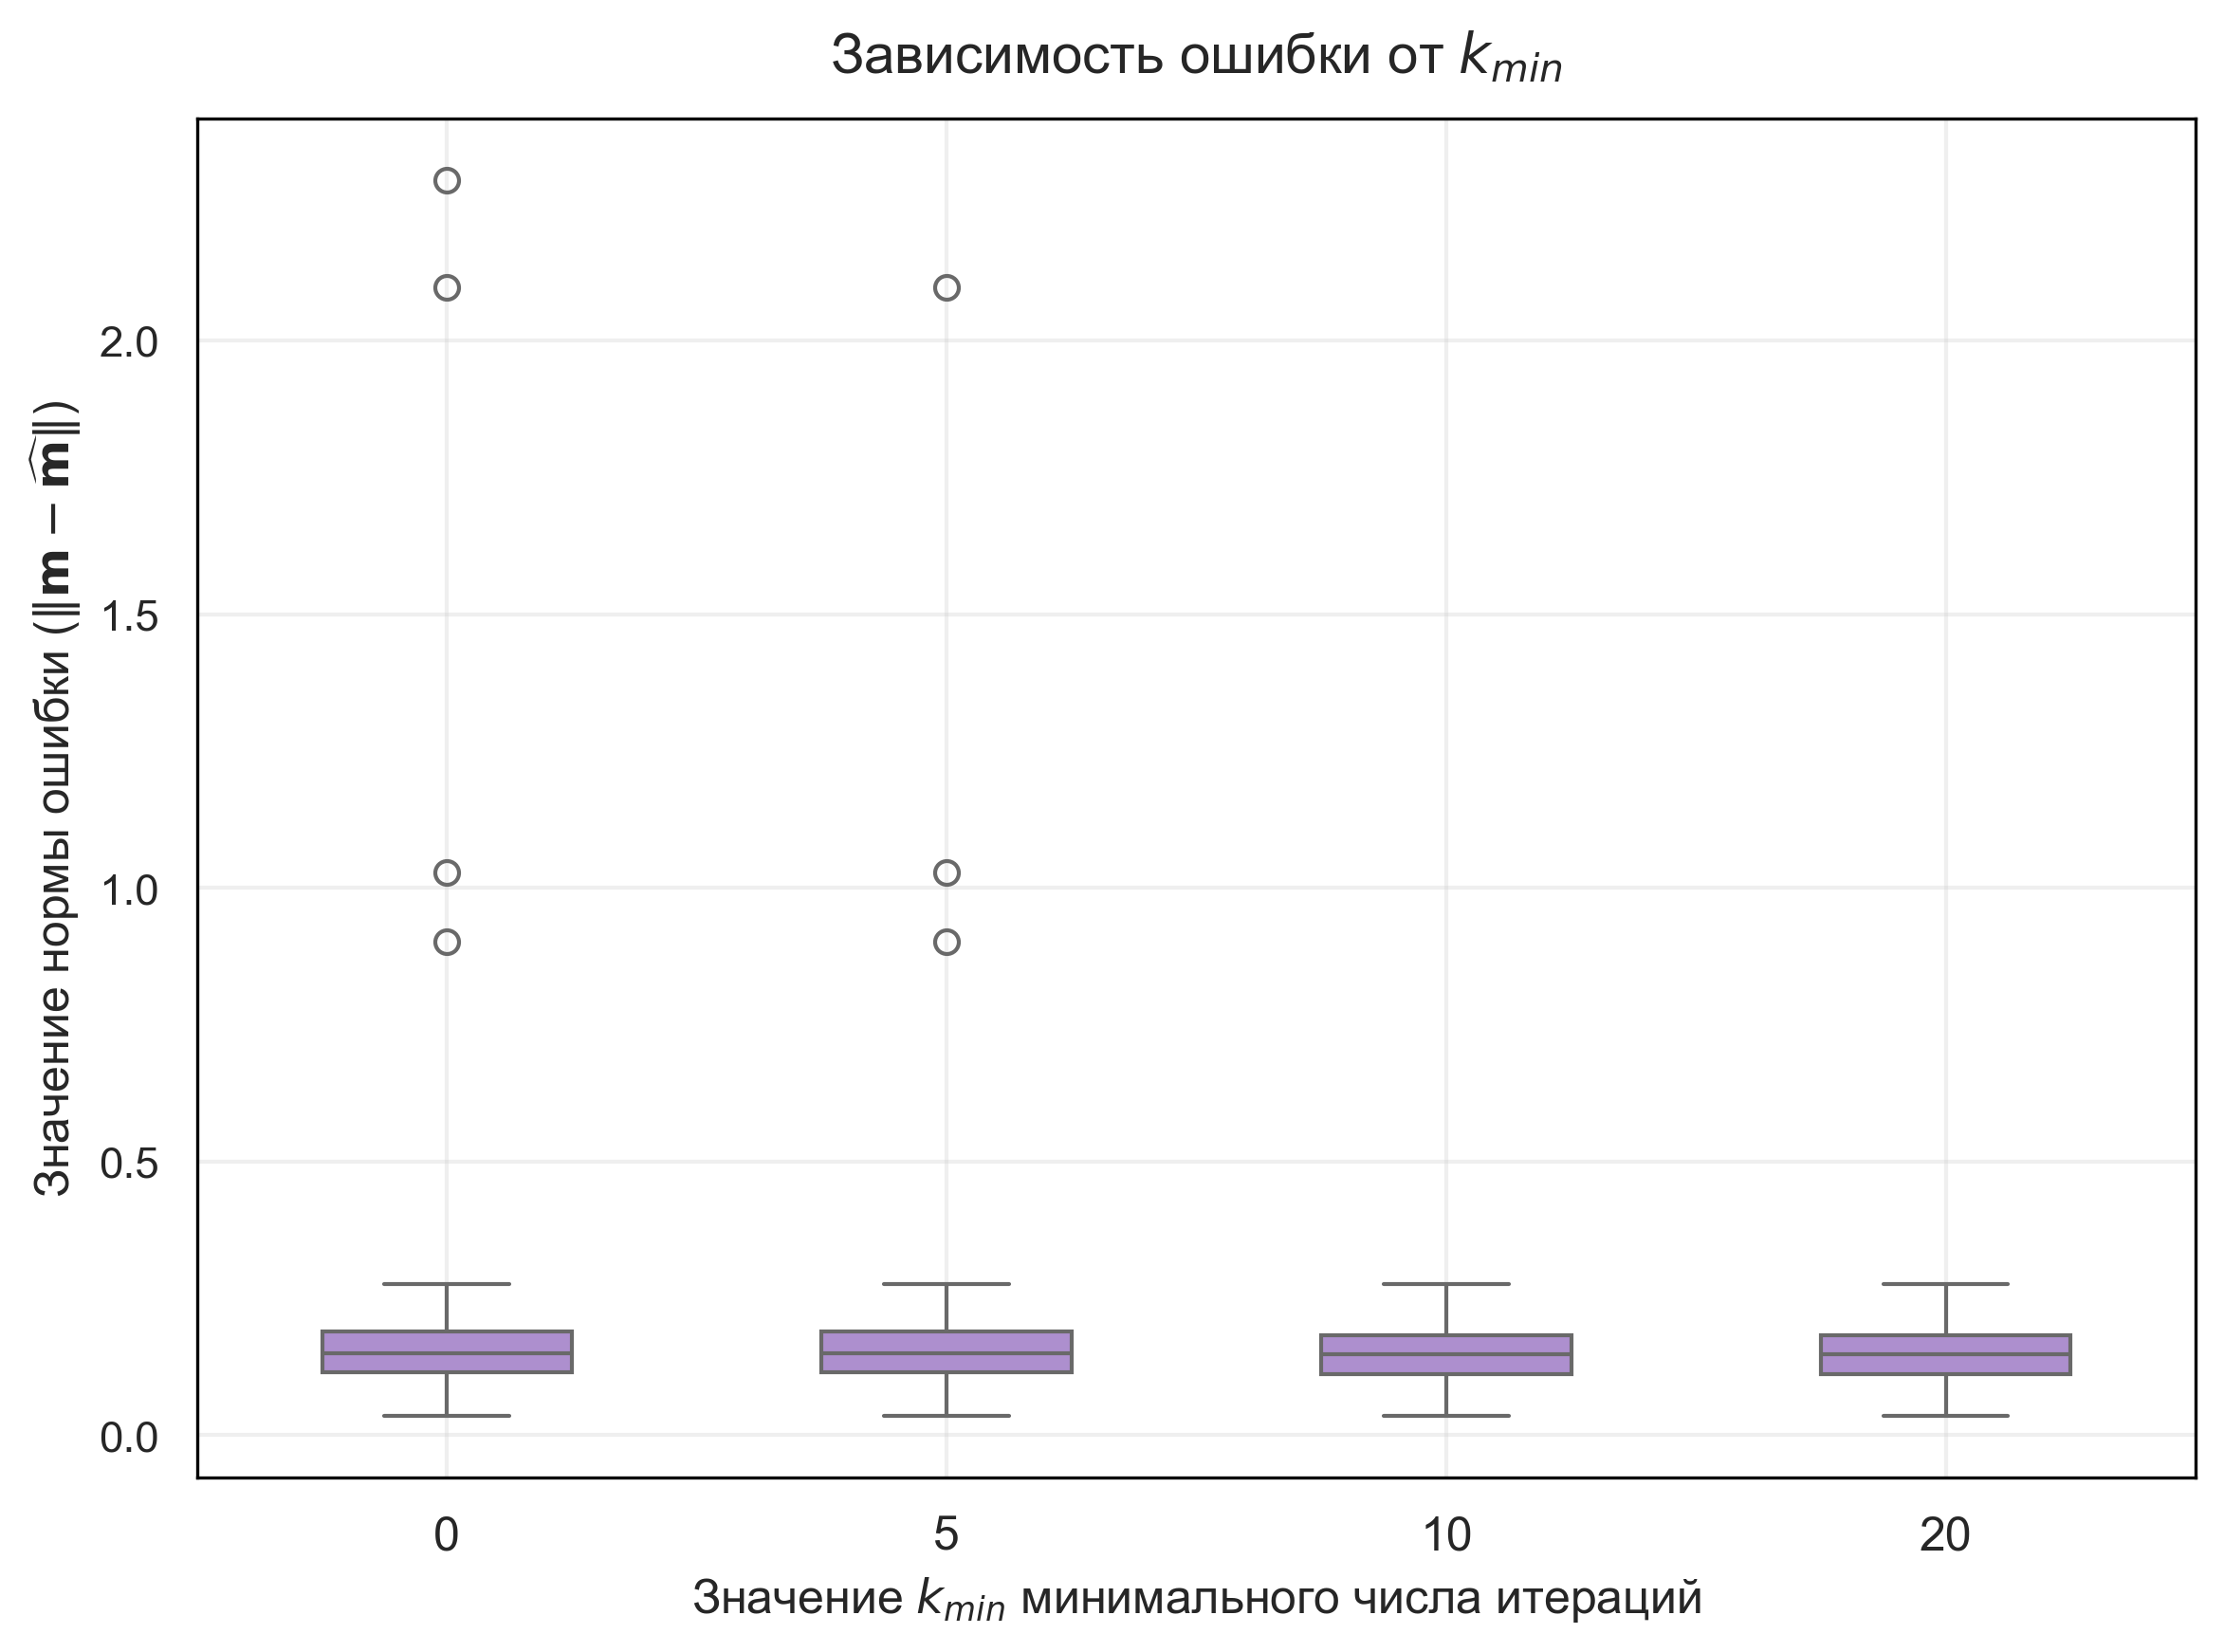
\includegraphics[width=0.8\textwidth]{stochastic_median_k_min_boxplots.png}
  \caption{Распределения ошибок модификации алгоритма для различных значений минимального числа итераций $k_{min}\in\{0,5,10,20\}$.}
  \label{fig:k_min}
\end{figure}

Видно, что увеличение минимального числа итераций практически не влияет на медианное значение ошибки и межквартильный размах распределения. Однако при $k_{min}=0$ и $k_{min}=5$ наблюдаются выбросы, соответствующие случаям преждевременной остановки алгоритма. При $k_{min}\geqslant 10$ подобные выбросы исчезают. 

Таким образом, введение минимального числа итераций позволяет существенно уменьшить вероятность крупных ошибок, связанных с преждевременной остановкой алгоритма, при этом практически не изменяя основные характеристики распределения ошибок.

\subsection{Многократное выполнение критерия останова}

В предыдущем разделе было показано, что введение минимального числа итераций позволяет уменьшить количество крупных ошибок, возникающих из-за преждевременной остановки алгоритма. Однако случайное выполнение критерия останова все еще возможно до достижения реальной сходимости.

Для дальнейшего повышения устойчивости рассмотрим следующую модификацию: алгоритм завершается только после того, как критерий останова выполнится  $c$ раз.

Пусть $c$ --- число выполнений критерия останова, необходимых для завершения алгоритма. На каждой итерации проверяется условие $\|\widehat{\mathbf{m}}_{{i}}-\widehat{\mathbf{m}}_{{i+1}}\|<\varepsilon \cdot \|\widehat{\mathbf{m}}_{{i}}\|$, если оно выполнено, то счетчик успешных проверок увеличивается на единицу. Алгоритм завершается только тогда, когда число выполнений критерия достигает значения $c$.

При $c=1$ получаем исходный вариант алгоритма с относительным критерием останова. Таким образом, данная модификация является естественным обобщением предыдущего подхода.

Рассмотрим работу алгоритма для значений $c\in\{1, 2, 3, 4, 5\}$.

\begin{figure}[!h]
   \centering
    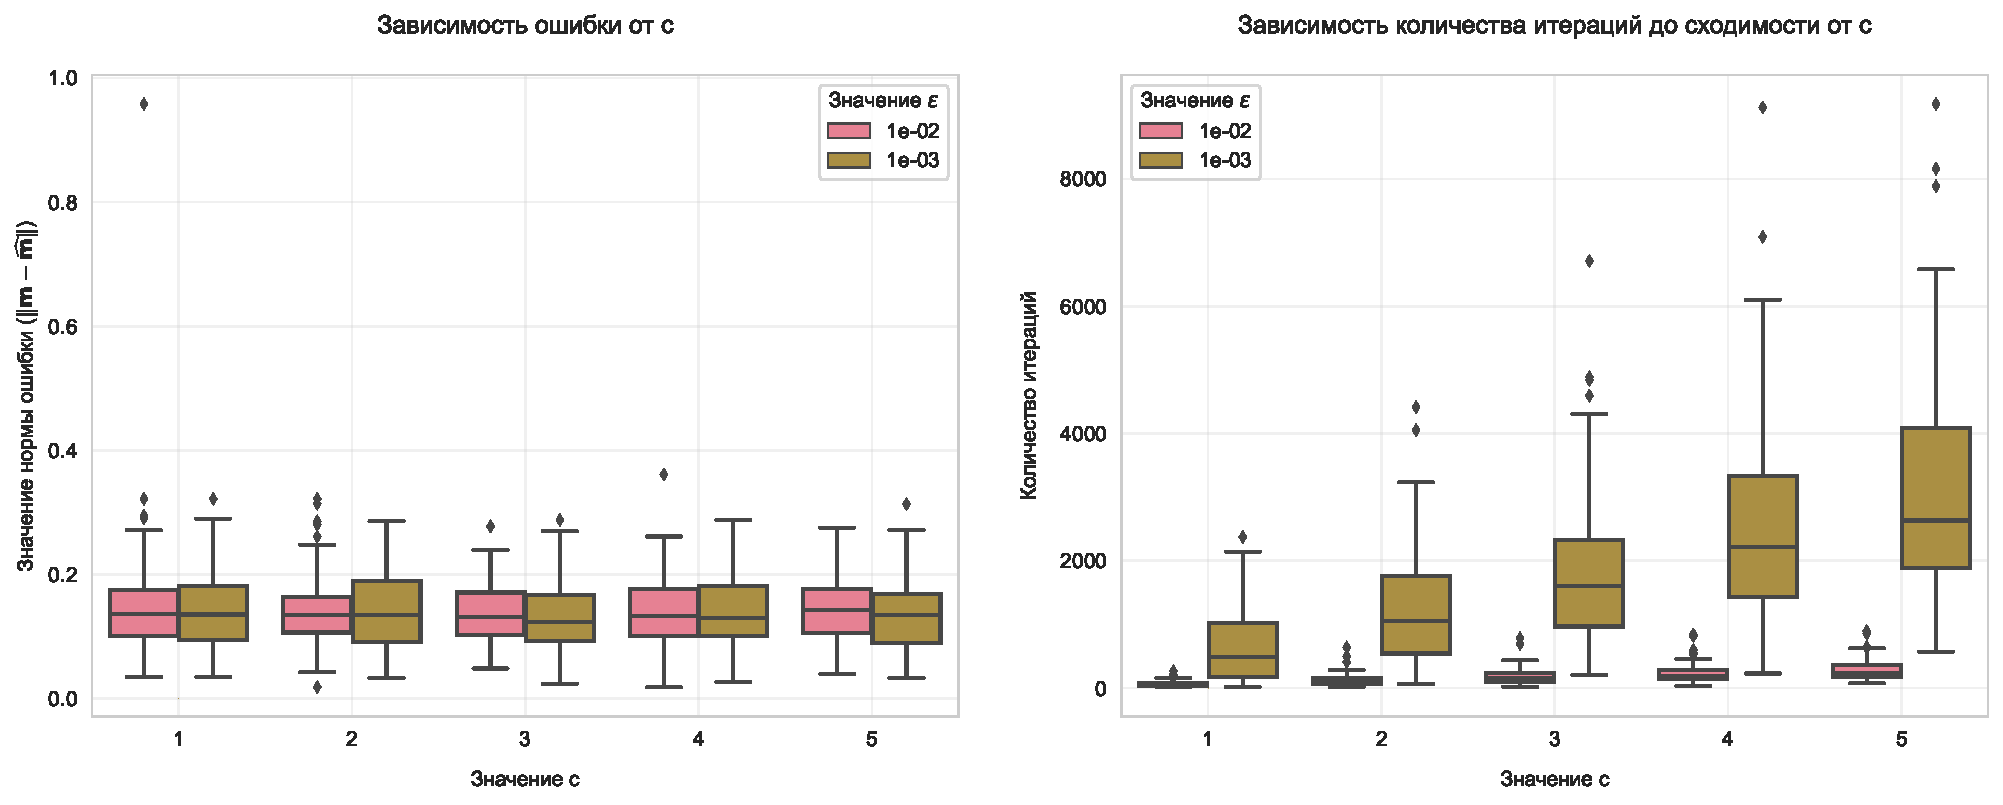
\includegraphics[width=15cm]{comp_stable_crit_results_out_5.pdf}
  \caption{Распределения ошибок и числа итераций для различных значений параметра $c$, где $c\in\{1, 2, 3, 4, 5\}$ --- число выполнений критерия останова, необходимых для завершения алгоритма.}
  \label{fig:comp_stable_crit_results_out_5}
\end{figure}

Результаты, представленные на рисунке~\ref{fig:comp_stable_crit_results_out_5}, показывают, что увеличение параметра $c$ позволяет практически устранить случаи преждевременной остановки алгоритма, приводящие к значительным ошибкам.  Однако точность при таком подходе повышается совсем незначительно. 

Также видно, что с ростом $c$ существенно увеличивается число итераций, необходимое для завершения алгоритма. Однако уменьшения разброса ошибок при больших значениях $c$ практически не наблюдается. Поэтому в данном случае использование значений $c>3$ оказывается практически неоправданным.

\section{Повышение точности оценки}

Предыдущие модификации были направлены прежде всего на повышение устойчивости алгоритма и уменьшение вероятности преждевременной остановки. Однако даже после достижения критерия останова финальная оценка все еще существенно зависит от случайного выбора направлений. Кроме того, вблизи оптимума последовательные приближения алгоритма начинают колебаться около истинного параметра положения. Поэтому использование только последней итерации может приводить к дополнительному разбросу оценки.

В данном разделе рассматриваются модификации, направленные непосредственно на повышение точности финальной оценки.

\subsection{Усреднение последних итераций}

Данная модификация основана на усреднении нескольких последних приближений алгоритма. Вместо использования результата последней итерации Алгоритма~\ref{alg:median} предлагается после достижения заданной точности $\varepsilon$ выполнить еще ${\text{w}}$ итераций и усреднить полученные оценки.

Пусть $N$ --- число итераций, необходимое для достижения критерия останова в Алгоритме~\ref{alg:median}, а ${\text{w}}$ --- число усредняемых итераций. Получаем последовательность приближений $\{\widehat{\mathbf{m}}_{{i}}\}_{i=N+1}^{N+{\text{w}}}$. Финальная оценка вычисляется по формуле
\[\widehat{\mathbf{m}}_{\text{avg}_{\text{w}}} = \frac{1}{{\text{w}}} \sum_{i=N+1}^{N+{\text{w}}} \widehat{\mathbf{m}}_{{i}}. \]


Усреднение последних итераций позволяет уменьшить влияние случайных колебаний отдельных итераций, тем самым снижая разброс финальной оценки.

Для исследования влияния параметра ${\text{w}}$ рассмотрим значения \\
${\text{w}}\in\{0,5,10,20\}$, где ${\text{w}}=0$ соответствует исходному алгоритму без усреднения.

На Рисунке~\ref{fig:additional_steps_boxplots} представлены распределения нормы ошибки для различных значений параметра ${\text{w}}$.

Видно, что увеличение числа усредняемых итераций приводит к уменьшению медианного значения ошибки, а также к небольшому уменьшению межквартильного размаха распределения. При этом наиболее заметное улучшение наблюдается при переходе от ${\text{w}}=0$ к ${\text{w}}=5$.

\begin{figure}[!hhh]
   \centering
    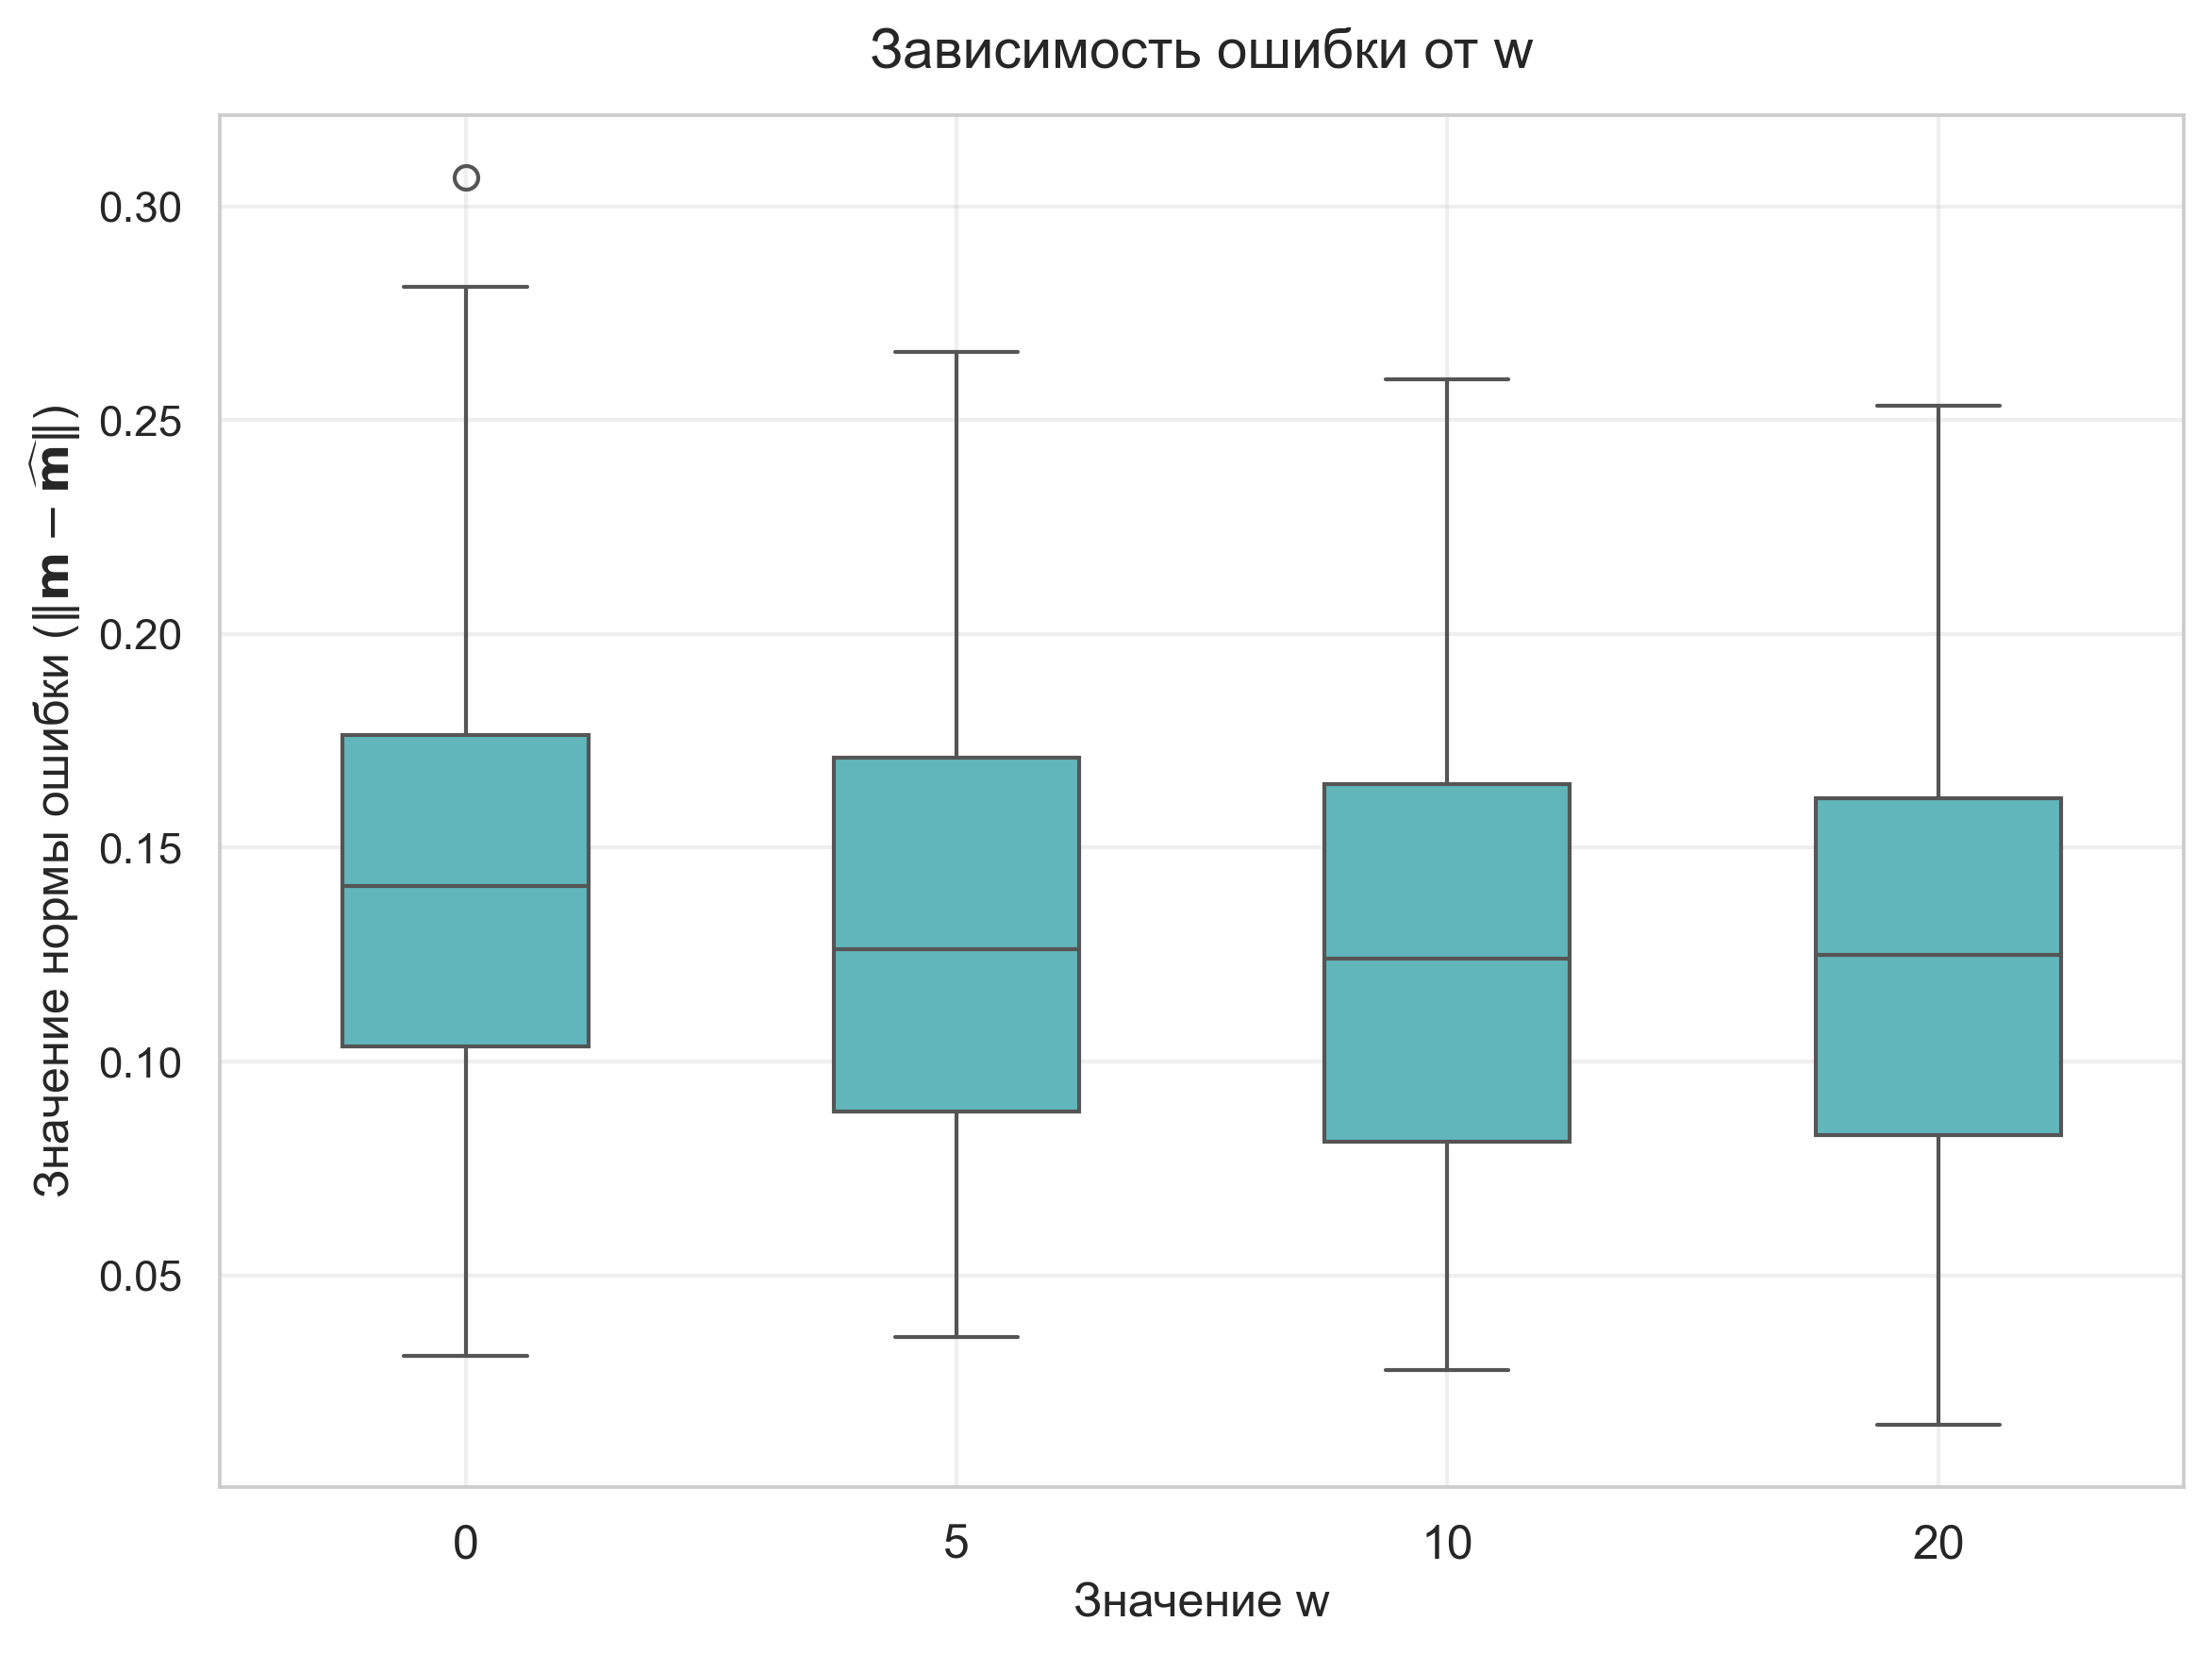
\includegraphics[width=0.8\textwidth]{stochastic_median_additional_steps_boxplots.png}
  \caption{Распределения ошибок модификации алгоритма для различных значений  $\text{w}\in\{0,5,10,20\}$, где ${\text{w}}$ --- число усредняемых последних итераций.}
  \label{fig:additional_steps_boxplots}
\end{figure}

Дальнейшее увеличение параметра ${\text{w}}$ продолжает уменьшать ошибку, однако эффект становится значительно менее выраженным. Таким образом, усреднение последних итераций позволяет повысить точность оценки за счет уменьшения влияния случайных колебаний алгоритма вблизи оптимума.

\subsection{Добавление экспоненциального сглаживания}

Усреднение последних итераций позволяет уменьшить влияние случайных колебаний алгоритма, однако требует выполнения дополнительных итераций уже после достижения критерия останова. Поэтому далее рассмотрим модификацию, изменяющую саму траекторию алгоритма и позволяющую стабилизировать процесс сходимости уже в ходе вычислений.

Для этого предлагается использовать экспоненциальное сглаживание, при котором новое приближение вычисляется как взвешенная комбинация текущей и предыдущей точек траектории.

Пусть последовательность $\widetilde{\mathbf{m}}_i$ задаёт сглаженную траекторию алгоритма, $\widehat{\mathbf{m}}_i$ --- шаг, вычисленный по Алгоритму~\ref{alg:median} из точки $\widetilde{\mathbf{m}}_{i-1}$. Тогда  новое приближение определяется по формуле
\begin{equation}\label{eq:smoothing}
{\widetilde{\mathbf{m}}}_i = \alpha {\widehat{\mathbf{m}}}_i + (1-\alpha) {\widetilde{\mathbf{m}}}_{i-1}, \quad 0 < \alpha \leqslant 1,   
\end{equation}
\vspace{-5ex}

\noindent{где $\alpha$ --- фиксированный параметр сглаживания.} 

Случай $\alpha = 1$ соответствует отсутствию сглаживания. Чем меньше значение $\alpha$, тем сильнее влияние предыдущих приближений на текущую точку траектории.

На Рисунке~\ref{fig:comp_stable_crit_results_exp}  представлены результаты работы алгоритма с экспоненциальным сглаживанием для $\alpha  \in \{0{,}1, \, 0{,}2, \,  0{,}3\}$. Для каждого значения параметра $\alpha$ проводилось моделирование при $c \in\{1,2,\ldots,10\}$, где $c$ --- число  выполнений критерия останова.

Из Рисунка~\ref{fig:comp_stable_crit_results_exp} видно, что использование экспоненциального сглаживания позволяет уменьшить медианное значение ошибки по сравнению с предыдущими модификациями алгоритма.

Для $\alpha=0{,}3$ и $\alpha=0{,}2$ (Рисунки \ref{fig:comp_stable_crit_results_exp_07_03} и \ref{fig:comp_stable_crit_results_exp_08_02}) уменьшение ошибки происходит уже при малых значениях $c$.  Однако дальнейшее увеличение параметра $c$ практически не влияет на распределение ошибок, тогда как число итераций продолжает быстро расти. 

Для $\alpha=0{,}1$ при $\varepsilon=10^{-3}$  (Рисунок \ref{fig:comp_stable_crit_results_exp_09_01}) распределение ошибок становится достаточно <<компактным>> уже при малых значениях $c$, хотя отдельные выбросы все еще сохраняются.  При $\varepsilon=10^{-2}$ разброс ошибок заметно больше, однако постепенно уменьшается при увеличении $c$.

Также видно, что при $\alpha=0{,}1$ рост числа итераций происходит значительно медленнее, чем для больших значений параметра $\alpha$. Таким образом, меньшие значения $\alpha$ позволяют получить более устойчивое распределение ошибок при существенно меньших вычислительных затратах.

Наиболее устойчивые результаты наблюдаются при $\alpha=0{,}1$, $c=5$, $\varepsilon = 10^{-3}$. Для данной комбинации распределение ошибок практически перестает изменяться при дальнейшем увеличении $c$, тогда как вычислительные затраты продолжают расти.

% Анализ результатов показал, что использование $\alpha = 0,3$ и $\alpha =  0,2$ при $c \geqslant 5$ и $\varepsilon = 10^{-3}$ не приводит к существенному улучшению точности по сравнению с $\alpha = 0,1$, но при этом значительно увеличивает вычислительную сложность алгоритма за счет увеличения количества итераций. Однако при $c \leqslant 4$ данные комбинации обеспечивают заметно меньшую ошибку (приблизительно в 2 раза) по сравнению с $\alpha = 0,1$.

% При этом для $\alpha = 0,3$ медианная ошибка не превышает $0,25$ при любом значении $c$ и $\varepsilon$, однако наблюдаются значительные выбросы (максимальная ошибка достигает $2,5$), что не позволяет считать этот вариант оптимальным. Для точности $\varepsilon = 10^{-3}$ и $\alpha = 0,3$ или $\alpha = 0,2$ распределение ошибки стабилизируется, начиная с $c = 2$, но это достигается за счет увеличения количества итераций, что еще раз говорит о том, что данное значение параметра можно не рассматривать и остановить выбор на $\alpha = 0,1$. 

% Для $\alpha = 0,1$ оптимальное значение $c=5$ при точности  $\varepsilon =10^{-3}$, так как при $c > 5$ распределение ошибок практически не изменяется и остается в пределах от 0 до $0,25$. Значение $c = 4$ также можно рассматривать, однако в этом случае наблюдается незначительный выброс по точности.

\begin{figure}[!htbp]
   \centering
\begin{subfigure}[b]{0.99\textwidth}
    \centering
    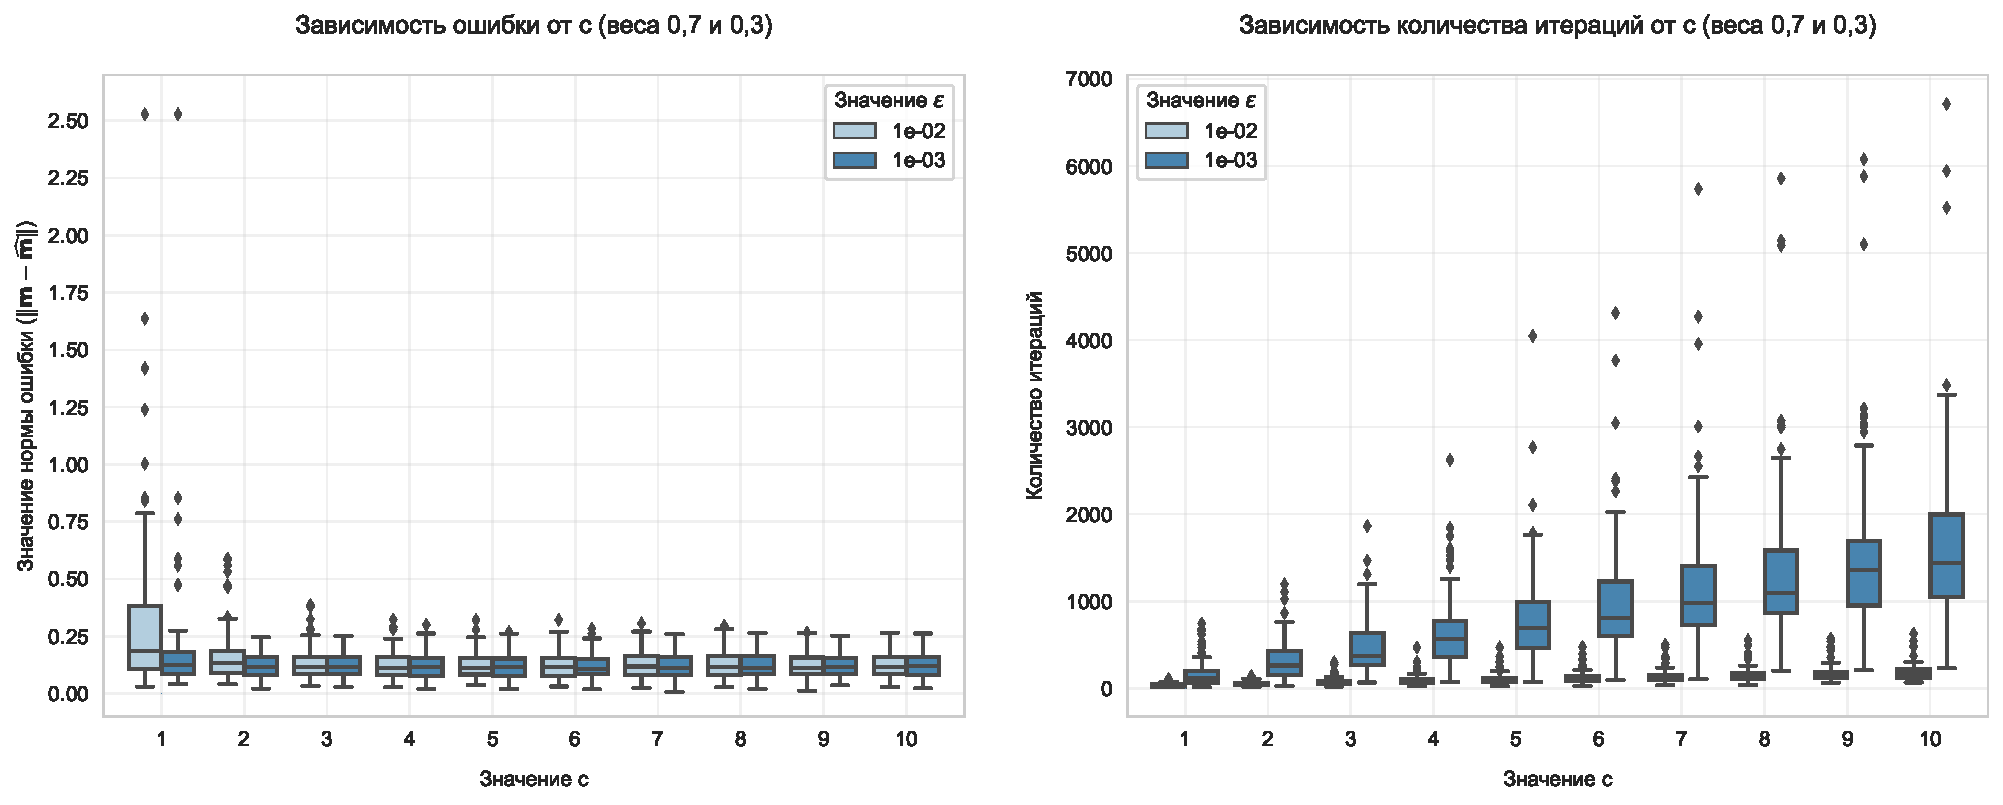
\includegraphics[width=\textwidth]{comp_stable_crit_results_exp_07_03.pdf}
    \captionsetup{labelformat=empty}
     \caption{(а) Распределение числа итераций и нормы ошибки для $\alpha = 0{,}3$}
    \label{fig:comp_stable_crit_results_exp_07_03}
  \end{subfigure}
  
   \vspace{1ex}
    
  \begin{subfigure}[b]{0.99\textwidth}
    \centering
    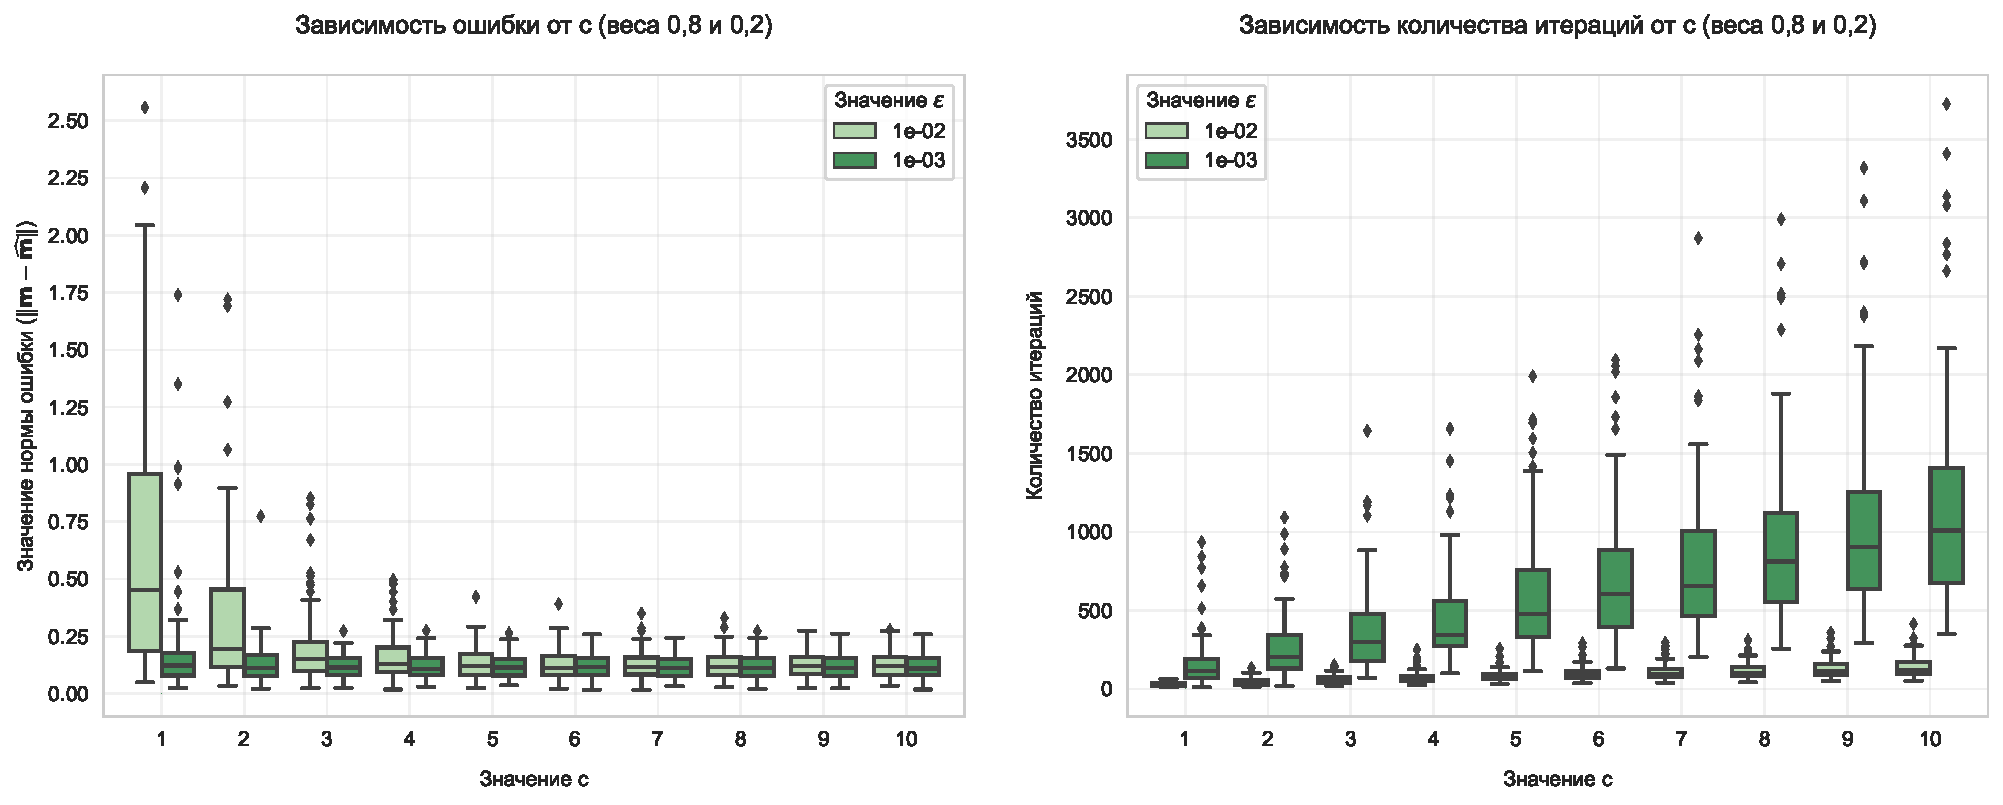
\includegraphics[width=\textwidth]{comp_stable_crit_results_exp_08_02.pdf}
    \captionsetup{labelformat=empty}
      \caption{(б) Распределение числа итераций и нормы ошибки для $\alpha = 0{,}2$}
    \label{fig:comp_stable_crit_results_exp_08_02}
  \end{subfigure}
  
   \vspace{1ex}
      
  \begin{subfigure}[b]{0.99\textwidth}
    \centering
    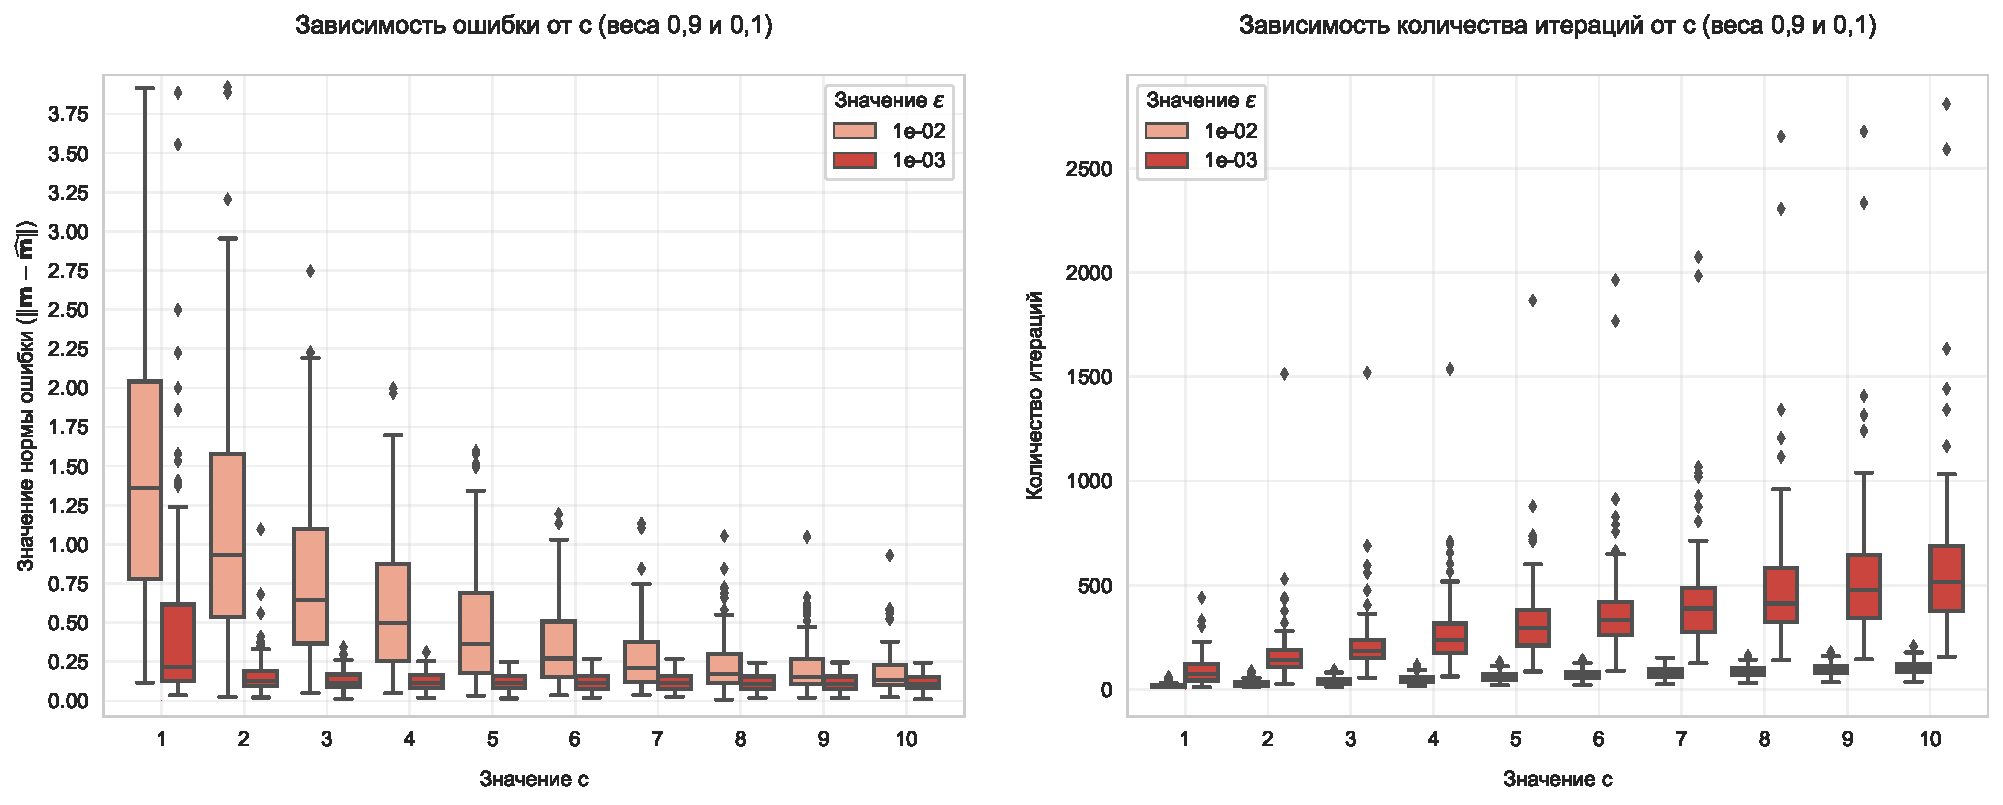
\includegraphics[width=\textwidth]{comp_stable_crit_results_exp_09_01.pdf}
    \captionsetup{labelformat=empty}
      \caption{(в) Распределение числа итераций и нормы ошибки для $\alpha = 0{,}1$}
    \label{fig:comp_stable_crit_results_exp_09_01}
  \end{subfigure}
  \caption{Результаты работы модификации алгоритма с экспоненциальным сглаживанием при различных значениях параметра сглаживания $\alpha$ и числа выполнений критерия останова $c$.
  }
  \label{fig:comp_stable_crit_results_exp}
\end{figure}


На Рисунке~\ref{fig:methods_comparison_exp_vs_avg} приведено сравнение метода с экспоненциальным сглаживанием при $\alpha =  0{,}1$ и $c=5$ (обозначен как  $\text{Exp Stable Rel Crit + Min It}$ на графике) и метода с усреднением последних итераций при ${\text{w}}=20$  с $c=5$  (обозначен как  $\text{Avg Stable Rel Crit + Min It}$ на графике). Видно, что использование экспоненциального сглаживания позволяет получить немного меньшую медианную ошибку и меньший разброс оценок. При этом сопоставимая точность достигается за существенно меньшее число итераций, что делает данный подход более вычислительно эффективным.

\begin{figure}[!htbp]
   \centering
    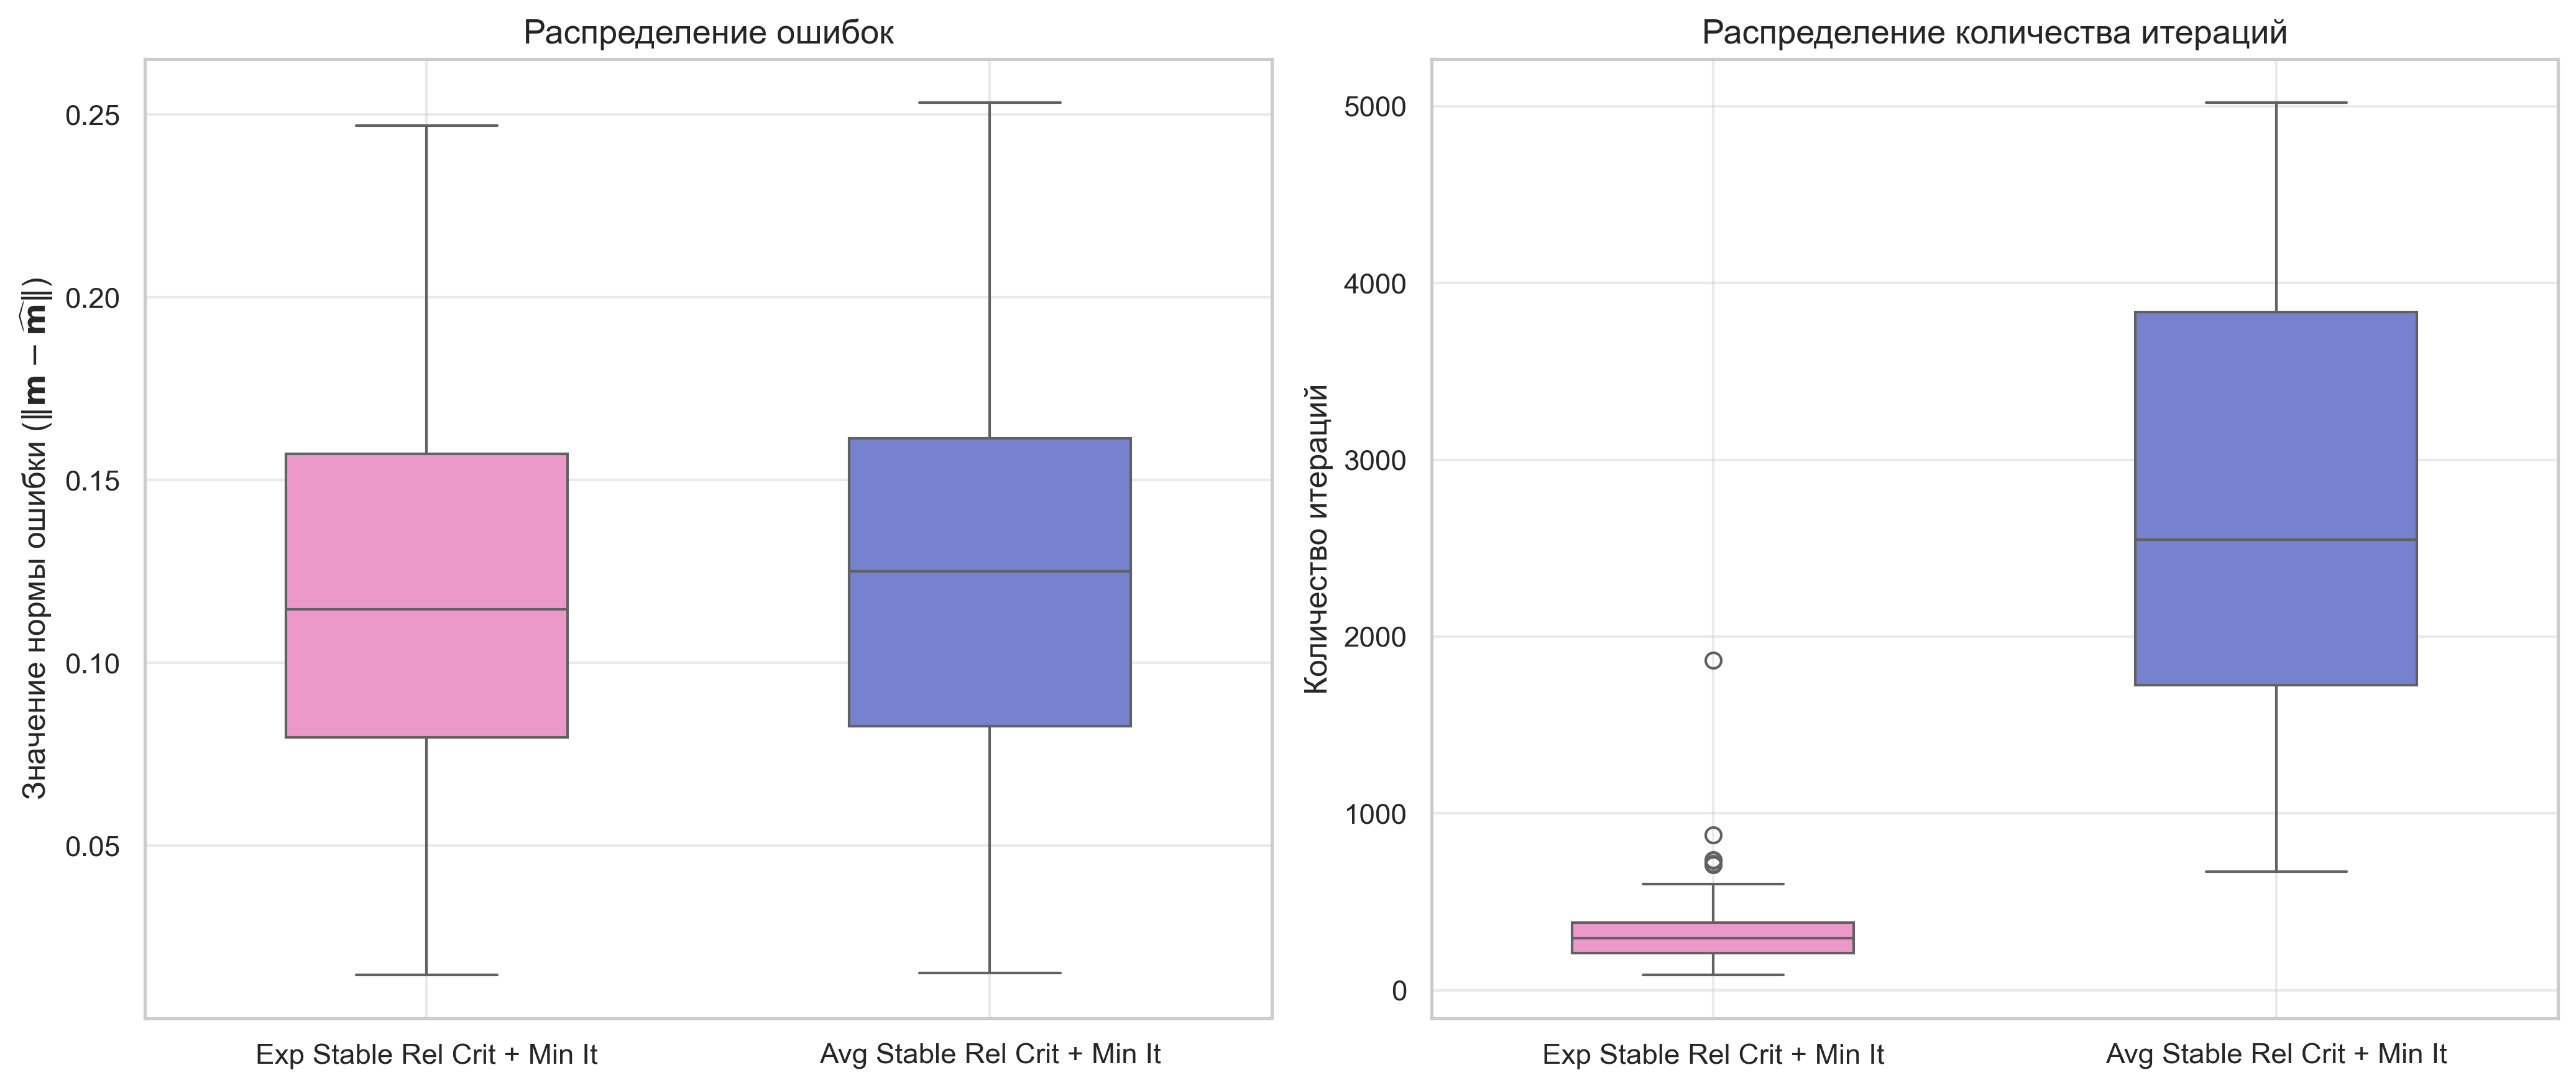
\includegraphics[width=1.01\textwidth]{methods_comparison_exp_vs_avg.png}
  \caption{Сравнение распределений ошибок и количества итераций для метода с усреднением последних итераций и метода с экспоненциальным сглаживанием. }
  \label{fig:methods_comparison_exp_vs_avg}
\end{figure}


\subsection{Применение адаптивного метода выбора шага к предложенному алгоритму}

В данном разделе предлагается посмотреть на предложенный Алгоритм~\ref{alg:median} как на метод, который совершает на итерации шаг вдоль вычисленного направления. Мы доказали в Теореме~\ref{eq:thetheorem}, что Алгоритм~\ref{alg:median} является частным случаем метода стохастического градиента, который, в свою очередь, является методом оптимизации вдоль выбранного направления. Предлагается перенять один подход из теории этих алгоритмов, который улучшает сходимость метода.


\subsubsection{Интерпретация алгоритма как метода оптимизации вдоль направления}

Пусть, как и в случае экспоненциального сглаживания в Алгоритме~\ref{alg:median} с поправкой \eqref{eq:smoothing}, $\widetilde{\mathbf{m}}_i$ обозначает текущее приближение медианы на $i$-й итерации, а $\widehat{\mathbf{m}}_i$ ~--- оценку медианы, полученную в результате проекции выборки на случайное направление, проходящее через $\widetilde{\mathbf{m}}_{i-1}$. Тогда обновление алгоритма можно записать в виде
\begin{equation}\label{eq:improvement_base}
\widetilde{\mathbf{m}}_{i+1} = \widetilde{\mathbf{m}}_i + \gamma_i (\widehat{\mathbf{m}}_{i+1} - \widetilde{\mathbf{m}}_i),
\end{equation}
где $\gamma_i > 0$ --- величина шага на $i$-й итерации. Вектор
\begin{equation}\label{eq:delta}
\delta_i = \widehat{\mathbf{m}}_{i+1} - \widetilde{\mathbf{m}}_i
\end{equation}
можно интерпретировать как направление шага, которое совершает метод. При $\gamma_i = \gamma = 1$ мы получаем стандартный Алгоритм~\ref{alg:median} без сглаживания, а при $\gamma_i = \gamma = \alpha$ из \eqref{eq:smoothing} получаем вариант с экспоненциальным сглаживанием.

Выбор $\alpha$, и, следовательно, $\gamma$ может быть затруднен для конкретной выборки. Предлагается рассмотреть подходы, в которых эта задача решается адаптивно, то есть, $\gamma = \gamma_i$ может меняться с итерацией.% Заметим, что при $\gamma_i = 1$ мы получаем базовый Алгоритм \ref{alg:median}, при $\gamma_i = \alpha$ --- вариант алгоритма с фиксированным экспоненциальным сглаживанием.


\subsubsection{Метод выбора длины шага, подобный AdaGrad}

Метод AdaGrad \cite{duchi2011adaptive} использует покоординатную адаптацию шага на основе накопленной суммы квадратов предыдущих стохастических градиентов. Однако, в контексте итерации~\eqref{eq:improvement_base} обновление принимает вид
\[
G_0 = 0 \in \mathbb{R}^d, \quad G_i = G_{i-1} + \delta_i \odot \delta_i,
\]
\[
\gamma_i = \min\left(1, \frac{\eta}{\sqrt{\sum_{j=1}^d G_j + \varepsilon}}\right),
\]
где $\odot$ обозначает покомпонентное умножение векторов, $\eta$ --- базовая величина шага, а $\varepsilon > 0$~--- малый регуляризационный параметр.

В оригинальной статье \cite{duchi2011adaptive} AdaGrad был введен как метод покомпонентного уточнения длины шага. Проблема в том, что прямое его применение к нашей задаче ухудшает сходимость, так как покомпонентное умножение вектора шага искажает его направление, и, как следствие, оценку параметра положения. Мы рассматриваем модификацию AdaGrad исключительно как метод адаптивного уменьшения длины шага для улучшения сходимости оценки.

\section{Численное сравнение рассмотренных модификаций}

В предыдущих разделах были рассмотрены различные модификации Алгоритма~\ref{alg:median}, направленные на повышение устойчивости и точности оценки. Далее проведем их численное сравнение.

Рассматриваются следующие методы:
\begin{itemize}
    \item алгоритм с относительным критерием останова ($\text{Rel Crit}$);
    
    \item алгоритм с относительным критерием останова и минимальным числом итераций ($\text{Rel Crit + Min It}$);
    
    \item алгоритм с многократным выполнением критерия останова ($\text{Stable Rel Crit}$);
    
    \item алгоритм с многократным выполнением критерия останова и минимальным числом итераций ($\text{Stable Rel Crit + Min It}$);
    
    \item алгоритм с усреднением последних итераций ($\text{Avg Stable Rel Crit + Min It}$);
    
    \item алгоритм с экспоненциальным сглаживанием ($\text{Exp Stable Rel Crit + Min It}$);
    
    \item алгоритм с адаптивным выбором шага на основе AdaGrad с базовым коэффициентом шага $\eta = 10$  ($\text{AdaGrad Stable Rel Crit + Min It}$).
\end{itemize}

Во всех экспериментах выборка объема $n = 1000$ генерировалась из трёхмерного нормального распределения $\mathcal{N}(\mathbf{m}, \mathbf{\Sigma} )$, где вектор математического ожидания $\mathbf{m}$ равен нулю, а в качестве ковариационной матрицы $\mathbf{\Sigma}$ взята матрица \eqref{eq:experimentmatrix}.

Для каждого метода проводилось $200$ независимых запусков алгоритма и рассчитывалась норма ошибки $\|\widehat{\mathbf{m}} - \mathbf{m}\|$, где $\widehat{\mathbf{m}}$ --- оценка медианы, полученная алгоритмом. Параметры у алгоритмов: $\varepsilon = 10^{-3}$, $k_{min}=10$, $c=5$, $\text{w}= 20$.

\vspace{1ex}

Сначала сравним модификации, направленные главным образом на повышение устойчивости алгоритма. Результаты представлены на рисунке~\ref{fig:error_distribution_base_minit_stable}.

\begin{figure}[!htbp]
		\centering
		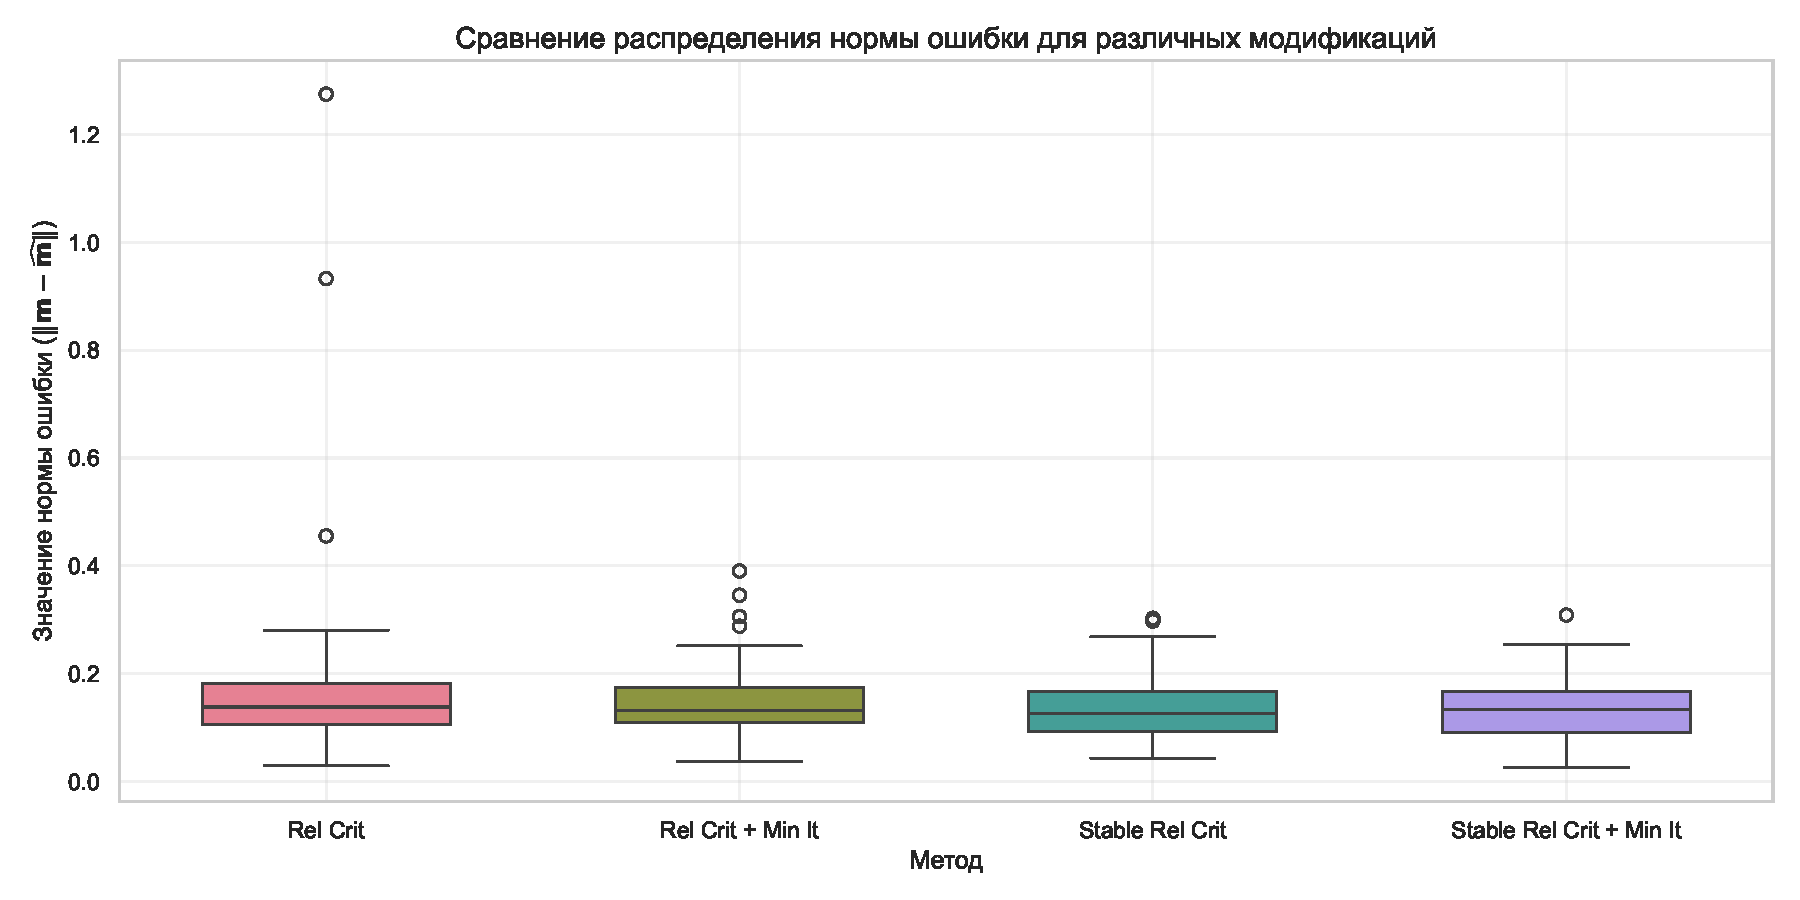
\includegraphics[width=0.9\textwidth]{error_distribution_base_minit_stable.pdf} 
		\caption{Распределения нормы ошибки для модификаций, основанных на изменении критерия останова.}
          \label{fig:error_distribution_base_minit_stable}
\end{figure}

На Рисунке~\ref{fig:error_distribution_base_minit_stable} видно, что использование минимального числа итераций и многократного выполнения критерия останова позволяет существенно уменьшить количество крупных выбросов ошибки по сравнению с алгоритмом, использующим только относительный критерий останова. 

При этом наименьший разброс ошибок наблюдается у метода $\text{Stable Rel Crit}$ + Min It, который сочетает обе модификации одновременно. Таким образом, комбинирование минимального числа итераций и многократного выполнения критерия останова позволяет заметно повысить устойчивость алгоритма.

\vspace{1.5ex}

Далее сравним модификации, изменяющие траекторию алгоритма и направленные непосредственно на повышение точности оценки. Результаты представлены на Рисунке~\ref{fig:error_distribution_ada_exp_avg}. 

\begin{figure}[!htbp]
    \centering
    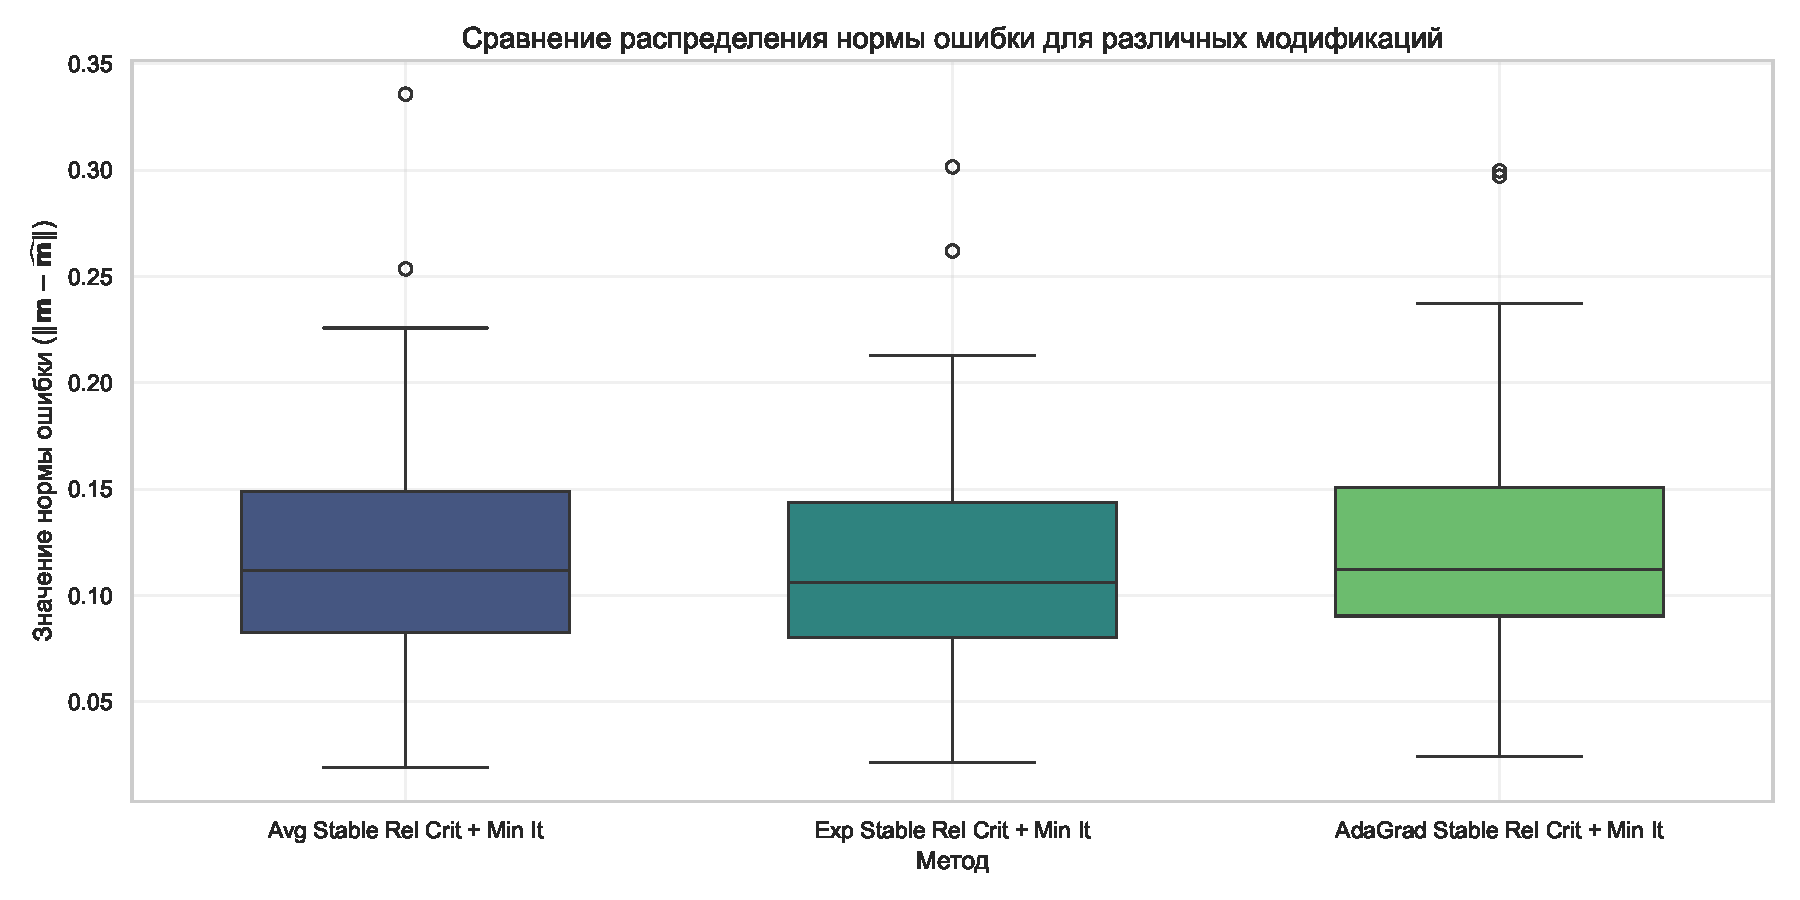
\includegraphics[width=0.9\textwidth]{error_distribution_ada_exp_avg.pdf}
    \caption{Распределения нормы ошибки для модификаций, изменяющих траекторию алгоритма.}
    \label{fig:error_distribution_ada_exp_avg}
\end{figure}

Из Рисунка~\ref{fig:error_distribution_ada_exp_avg} видно, что все три метода демонстрируют близкие результаты. Наибольший разброс ошибок наблюдается у метода с усреднением последних итераций.

Использование экспоненциального сглаживания позволяет немного уменьшить медианное значение ошибки и сделать распределение более компактным. Метод AdaGrad показывает сопоставимые результаты, однако его преимущества перед экспоненциальным сглаживанием оказываются менее выраженными для рассматриваемого распределения.

\vspace{1.5ex}

Наконец, сравним модификации, изменяющие траекторию алгоритма, с предыдущими модификациями критерия останова. Результаты представлены на Рисунке~\ref{fig:error_distribution_not_base}. 

% На Рисунке~\ref{fig:error_distribution_ada_exp_avg} представлены боксплоты распределений ошибок для всех рассматриваемых методов.

\begin{figure}[!htbp]
    \centering
    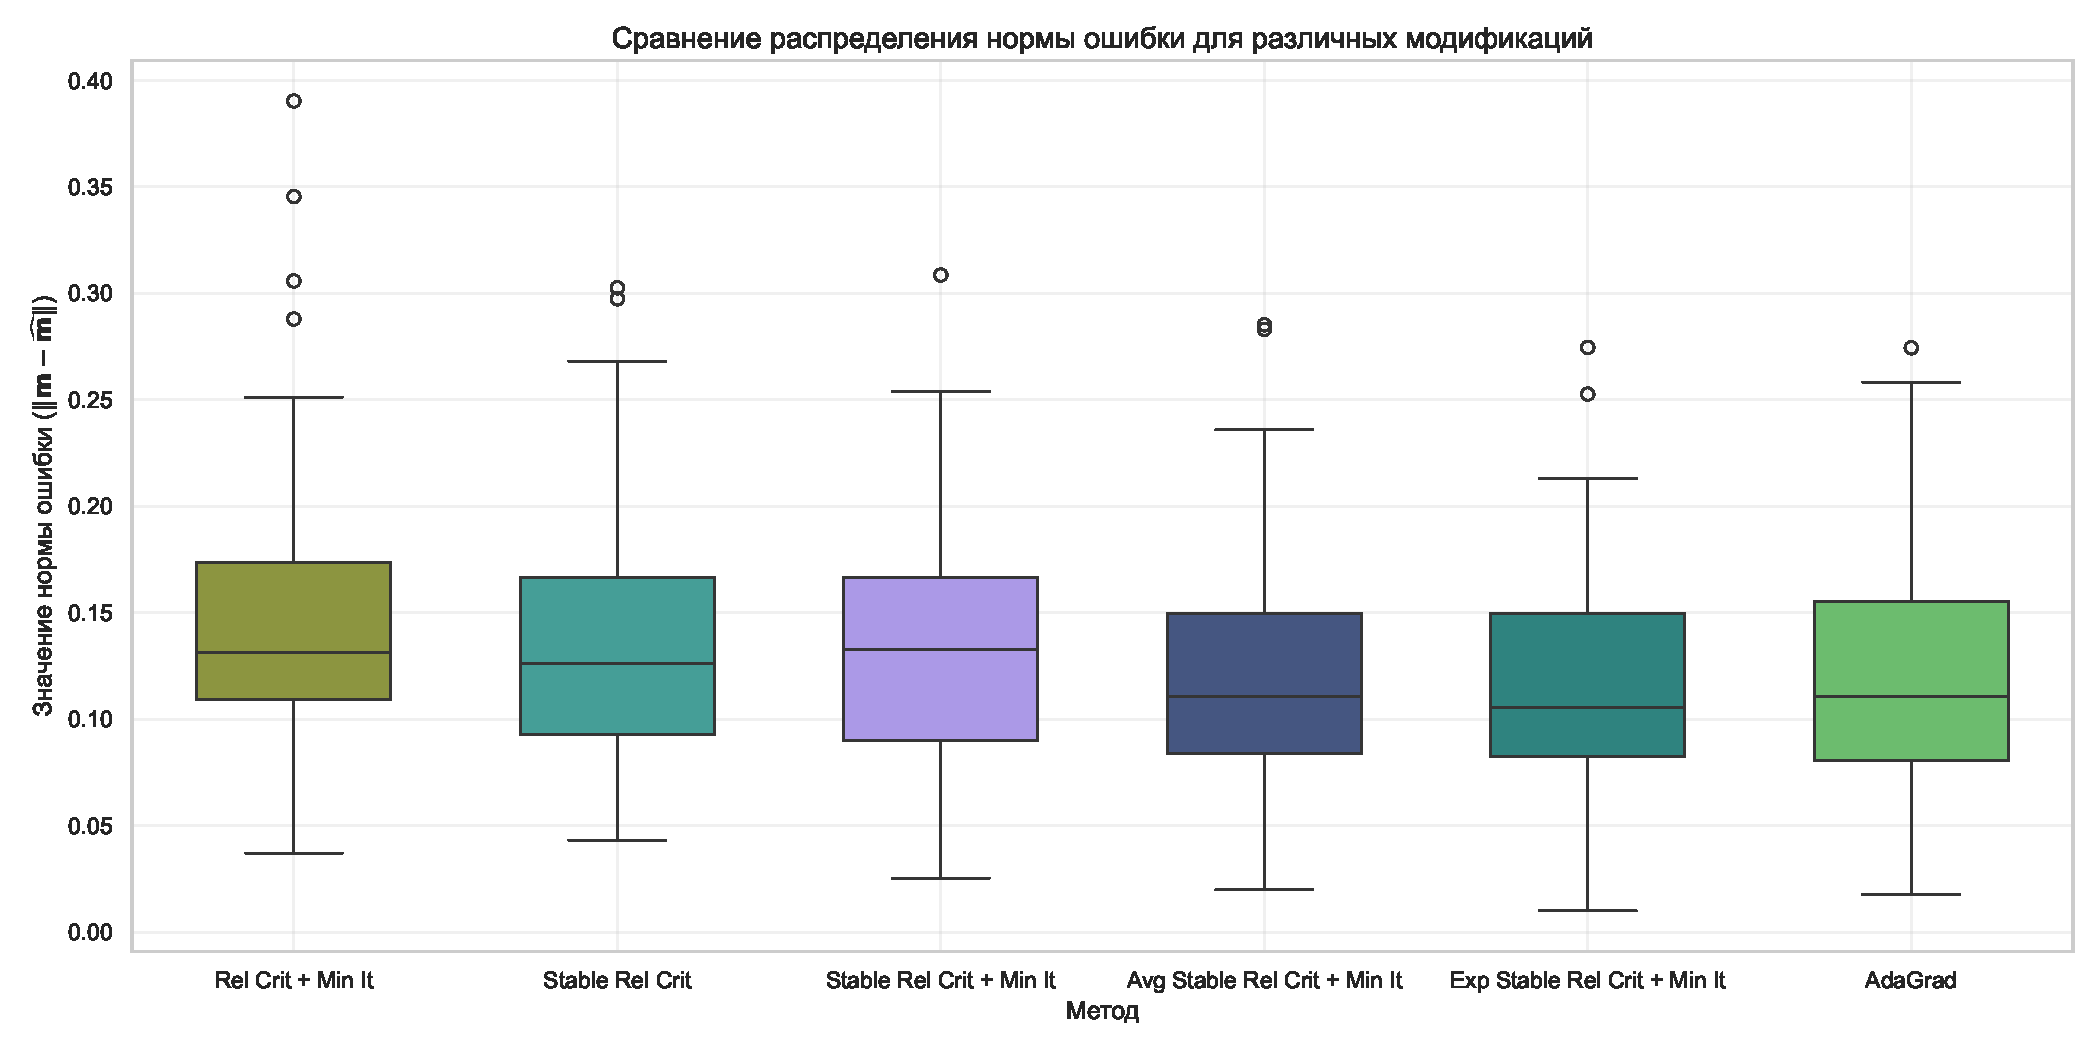
\includegraphics[width=0.9\textwidth]{error_distribution_not_base.pdf}
    \caption{Сравнение распределений нормы ошибки для различных модификаций алгоритма.}
    \label{fig:error_distribution_not_base}
\end{figure}


Из Рисунка~\ref{fig:error_distribution_not_base} видно, что модификации, изменяющие траекторию алгоритма, позволяют дополнительно уменьшить медианное значение ошибки по сравнению с методами, основанными только на изменении критерия останова.

Наиболее устойчивые результаты демонстрируют методы $\text{Exp Stable Rel Crit}$ + Min It и $\text{AdaGrad Stable Rel Crit + Min It}$. При этом метод с экспоненциальным сглаживанием показывает немного меньший разброс ошибок.

Таким образом, модификации траектории оказываются более эффективными для повышения точности оценки, чем модификации, связанные исключительно с критерием останова. В то же время методы, основанные на изменении критерия останова, существенно повышают устойчивость алгоритма и уменьшают вероятность появления крупных ошибок.


\section{Исследование робастности модификаций алгоритма}

Помимо точности и устойчивости алгоритма, важным свойством рассматриваемых методов является робастность. В работе~\cite{filatova2024robust} было показано, что базовый Алгоритм~\ref{alg:median} устойчив к наличию выбросов. Однако добавление модификаций, изменяющих критерий останова и траекторию сходимости, может влиять на данное свойство. Поэтому далее исследуется, как различные модификации алгоритма ведут себя при увеличении доли выбросов в выборке.

Во всех экспериментах использовались те же данные, что и в предыдущем разделе: выборки объема $n=1000$ генерировались из трехмерного нормального распределения с $\mathbf{m}=\mathbf{0}$ и ковариационной матрицей \eqref{eq:experimentmatrix}.

Для исследования робастности часть наблюдений в выборке заменялась на точку-выброс $(100; 100; 100)^{\mathrm T}$ с весом $\{0\%,\,5\%,\,10\%,\,15\%,\,20\%,\,25\%\}.$

Для каждого метода проводилось $200$ независимых запусков алгоритма и рассчитывалась норма ошибки $\|\widehat{\mathbf{m}} - \mathbf{m}\|$, где $\widehat{\mathbf{m}}$ --- оценка параметра положения, полученная алгоритмом.

В сравнение также была включена геометрическая медиана, поскольку, как отмечалось ранее, именно она является основным конкурентом предложенного алгоритма с точки зрения точности и вычислительной эффективности.

На Рисунке~\ref{fig:location_error_dependency} представлена зависимость средней ошибки оценки параметра положения от веса точки-выброса для различных модификаций алгоритма.

\begin{figure}[!htbp]
    \centering
    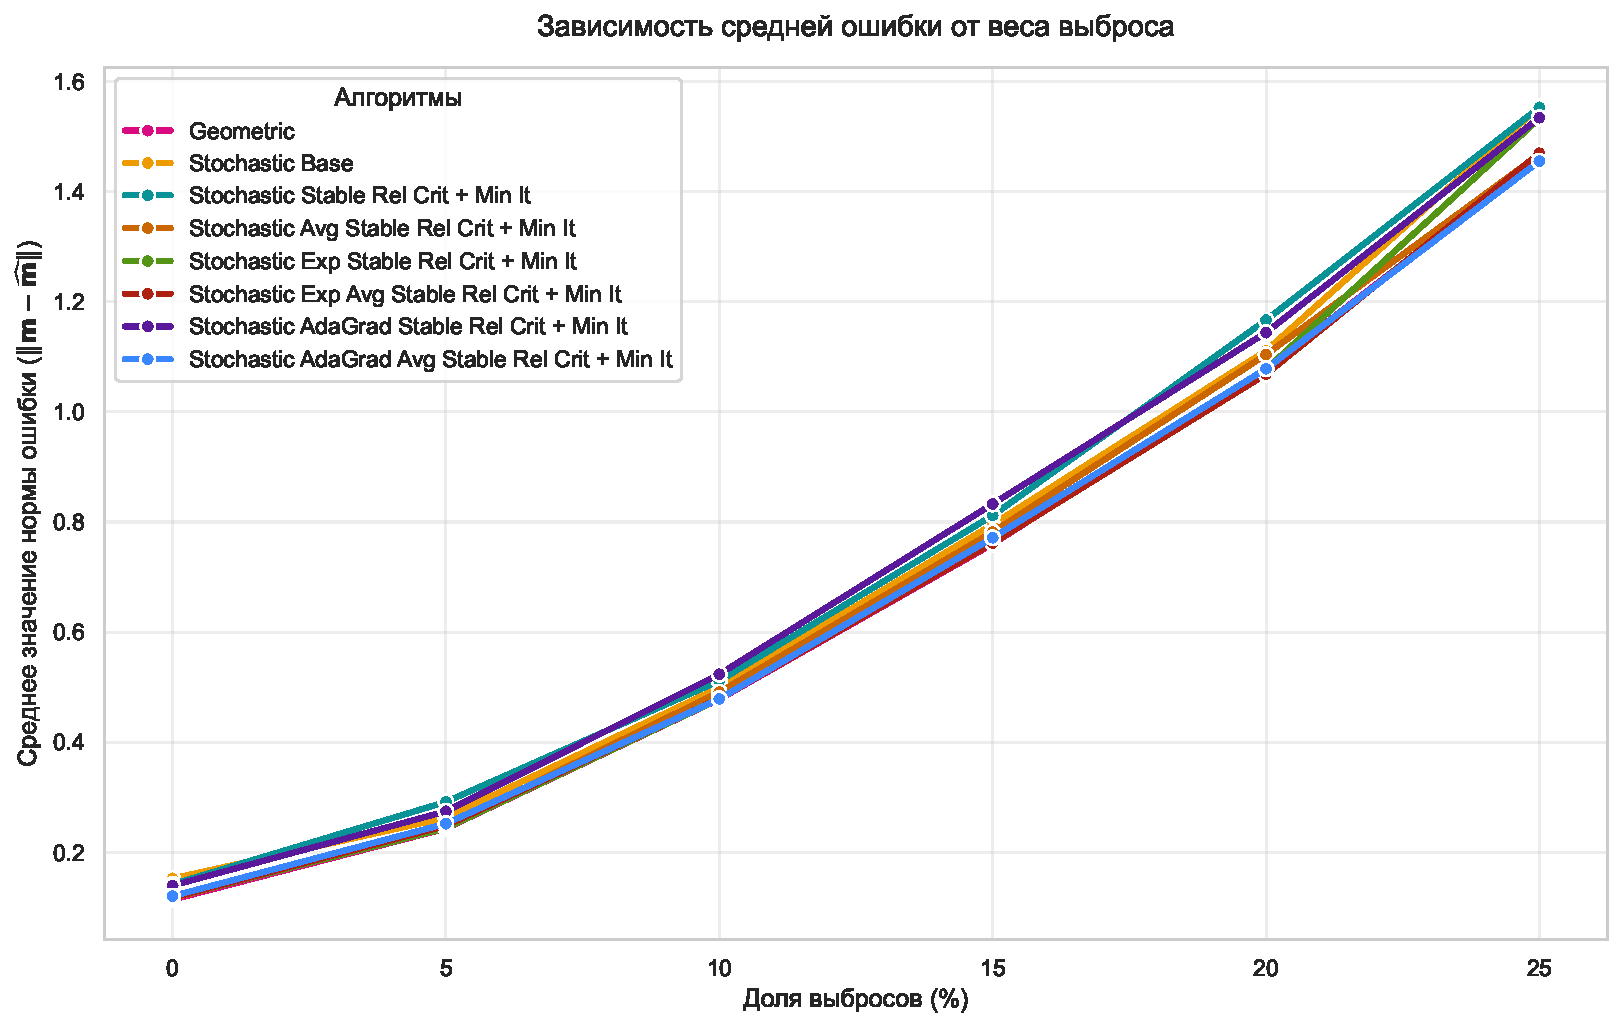
\includegraphics[width=0.9\textwidth]{location_error_dependency.pdf}
    \caption{Зависимость средней нормы ошибки от веса точки-выброса для различных модификаций алгоритма.}
    \label{fig:location_error_dependency}
\end{figure}

Из Рисунка~\ref{fig:location_error_dependency} видно, что для всех рассматриваемых методов ошибка монотонно возрастает с увеличением веса выброса. Однако различия между алгоритмами оказываются сравнительно небольшими.

Геометрическая медиана заметно не выделяется на этом графике, что говорит о том, что предложенный алгоритм сопаставим с ней по свойствам робасности.

Среди модификаций стохастического алгоритма наиболее устойчивые результаты показывают методы, использующие усреднение и сглаживание траектории. В частности, модификации Stochastic Exp Avg Stable Rel Crit и Stochastic AdaGrad Avg Stable Rel Crit демонстрируют немного меньшие значения ошибки по сравнению с базовыми версиями алгоритма. Тем не менее различия между методами остаются относительно небольшими даже при $20\%-25\%$ выбросов.

В целом эксперимент показывает, что предложенные модификации позволяют сохранить робастные свойства алгоритма при наличии выбросов, а использование сглаживания и усреднения траектории позволяет дополнительно уменьшить ошибку оценки параметра положения.

